\documentclass{article}
\usepackage[authoryear, round]{natbib} % Citation format
\usepackage{hyperref}   % Hyperlink support
\usepackage{tcolorbox}
\usepackage{amsmath}    % Math formula support
\usepackage{amssymb}    % Math symbol support
\usepackage{amsfonts}   % Math font support
\usepackage{amsthm}     % Theorem environment support
\usepackage{booktabs}   % Table formatting support
\newtheorem{lemma}{Lemma}
\newtheorem{theorem}{Theorem}
\newtheorem{definition}{Definition}
\newtheorem{proposition}{Proposition}
\usepackage{algorithm, algorithmicx, algpseudocode} % Algorithm support
\usepackage{lmodern}
\usepackage{graphicx}   % Image support
\usepackage{listings}   % Code highlighting support
\usepackage{geometry}   % Page setup
\geometry{a4paper, margin=0.5in} % Set page size and margins
\usepackage{tikz} % TikZ drawing support
\usetikzlibrary{mindmap, shadings}
\usepackage{enumitem} % Enhanced list environments

\usepackage{xcolor}    % Color support
\definecolor{lightgray}{gray}{0.90} % Light gray
\definecolor{commentgreen}{rgb}{0.161, 0.510, 0.322} % Define custom green
\definecolor{answercolor}{rgb}{0.0, 0.0, 0.8} % Blue for answers

\lstdefinestyle{pythonstyle}{
    language=Python,
    basicstyle=\ttfamily\small,
    keywordstyle=\color{blue},
    stringstyle=\color{red},
    commentstyle=\color{commentgreen},
    morecomment=[l][\color{magenta}]{\#},
    showstringspaces=false,
    breaklines=true,
    frame=single,
    backgroundcolor=\color{lightgray!10},
    escapeinside={(*@}{@*)}, % allow LaTeX commands in code, e.g., (*@\textbf{bold}@*)
    literate={'}{\textquotesingle}1 % handle single quotes correctly
}

\lstset{style=pythonstyle} % Set the default style for listings

% Define answer environment
\newtcolorbox{answer}{
    colback=blue!5!white,
    colframe=blue!75!black,
    title=Answer,
    fonttitle=\bfseries,
    left=2mm,
    right=2mm,
    boxsep=1mm
}

\newtcolorbox{note}{
    colback=green!5!white,
    colframe=green!75!black,
    title=Note,
    fonttitle=\bfseries,
    left=2mm,
    right=2mm,
    boxsep=1mm
}

% Define problem counter and environment
\newcounter{problem}
\newcommand{\problem}[2]{
    \stepcounter{problem}
    \subsection{Problem (\texttt{#1}): #2}
    \vspace{-1.5em} % Reduce space after subsection
    \noindent
}

% Remove paragraph indentation and add spacing
\setlength{\parindent}{0pt}
\setlength{\parskip}{6pt}

\title{CS336 Assignment 1 Writeup}
\author{Linkang Dong}
\date{\today}

\begin{document}

\maketitle

% Add table of contents
\tableofcontents
\newpage

\section{Assignment Overview}
\vspace{-1em}

This document contains my solutions to CS336 Assignment 1. Each problem is answered in detail with supporting explanations, calculations, and code where applicable.
\section{Byte-Pair Encoding (BPE) Tokenizer}

\problem{unicode1}{Understanding Unicode (1 point)}

\begin{enumerate}[label=(\alph*)]
    \item {What Unicode character does \texttt{chr(0)} return?}
    
    {\textbf{Deliverable}: A one-sentence response.}
    
    \begin{answer}
    \texttt{chr(0)} returns the null byte \texttt{'\textbackslash x00'}.
    \end{answer}
    
    \item {How does this character's string representation (\texttt{\_\_repr\_\_()} differ from its printed representation?}
    
    {\textbf{Deliverable}: A one-sentence response.}
    
    \begin{answer}
    \texttt{chr(0).\_\_repr\_\_()} returns \texttt{'\textbackslash\textbackslash x00'}, adding a backslash \texttt{\textbackslash} before the \texttt{x}.
    \end{answer}
    
    \item {What happens when this character occurs in text? It may be helpful to play around with the following in your Python interpreter and see if it matches your expectations:}
    
    \begin{lstlisting}
>>> chr(0)
>>> print(chr(0))
>>> "this is a test" + chr(0) + "string"
>>> print("this is a test" + chr(0) + "string")
    \end{lstlisting}
    
    {\textbf{Deliverable}: A one-sentence response.}
    
    \begin{answer}
    It prints nothing when it occurs in text; the result is "this is a teststring".
    \end{answer}
\end{enumerate}

\problem{unicode2}{Unicode Encodings (3 points)}

\begin{enumerate}[label=(\alph*)]
    \item {What are some reasons to prefer training our tokenizer on UTF-8 encoded bytes, rather than UTF-16 or UTF-32? It may be helpful to compare the output of these encodings for various input strings.}
    
    {\textbf{Deliverable}: A one-to-two sentence response.}
    
    \begin{answer}
    UTF-8 is more space-efficient for texts that are primarily in ASCII, as it uses one byte for these characters, while UTF-16 and UTF-32 use two and four bytes respectively; additionally, UTF-8 is backward compatible with ASCII and is the most widely used encoding on the web (more than 98\% of all webpages).
    \end{answer}
    
    \item {Consider the following (incorrect) function, which is intended to decode a UTF-8 byte string into a Unicode string. Why is this function incorrect? Provide an example of an input byte string that yields incorrect results.}
    
    \begin{lstlisting}
def decode_utf8_bytes_to_str_wrong(bytestring: bytes):
    return "".join([bytes([b]).decode("utf-8") for b in bytestring])
    \end{lstlisting}
    
    \begin{lstlisting}
>>> decode_utf8_bytes_to_str_wrong("hello".encode("utf-8"))
'hello'
    \end{lstlisting}
    
    {\textbf{Deliverable}: An example input byte string for which \texttt{decode\_utf8\_bytes\_to\_str\_wrong} produces incorrect output, with a one-sentence explanation of why the function is incorrect.}
    
    \begin{lstlisting}
>>> "hello".encode("utf-8")
b'hello'
>>> "hello".encode("utf-8").decode("utf-8")
'hello'
>>> decode_utf8_bytes_to_str_wrong("hello".encode("utf-8"))
'hello'
>>> "é".encode("utf-8")
b'\xc3\xa9'
>>> "é".encode("utf-8").decode("utf-8")
'é' 
>>> decode_utf8_bytes_to_str_wrong("é".encode("utf-8"))
Traceback (most recent call last):
  File "<stdin>", line 1, in <module>
  File "<stdin>", line 2, in decode_utf8_bytes_to_str_wrong
UnicodeDecodeError: 'utf-8' codec can't decode byte 0xc3 in position 0: unexpected end of data
    \end{lstlisting}

    \begin{answer}
    An example input byte string is \texttt{b'\textbackslash xc3\textbackslash xa9'}, which represents the character 'é' in UTF-8. The function is incorrect because \textbf{it decodes each byte individually}, leading to a \texttt{UnicodeDecodeError} since \texttt{b'\textbackslash xc3'} and \texttt{b'\textbackslash xa9'} are not valid standalone UTF-8 characters.
    \end{answer}
    
    \item {Give a two byte sequence that does not decode to any Unicode character(s).}
    
    {\textbf{Deliverable}: An example, with a one-sentence explanation.}
    
    \begin{lstlisting}
>>> b'\x80\x80'.decode("utf-8") 
Traceback (most recent call last):
  File "<stdin>", line 1, in <module>
UnicodeDecodeError: 'utf-8' codec can't decode byte 0x80 in position 0: invalid start byte
    \end{lstlisting}

    \begin{answer}
    The byte sequence \texttt{b'\textbackslash x80\textbackslash x80'} does not decode to any Unicode characters because it is an invalid UTF-8 sequence; in UTF-8, continuation bytes (bytes starting with \texttt{10xxxxxx}) must follow a valid leading byte, and \texttt{0x80} cannot be a leading byte.
    \end{answer}
\end{enumerate}

\problem{train\_bpe}{BPE Tokenizer Training (15 points)}

Write a function that, given a path to an input text file, trains a (byte-level) BPE tokenizer. Your BPE training function should handle (at least) the following input parameters:

\begin{itemize}
    \item \lstinline{input_path: str} - Path to a text file with BPE tokenizer training data.
    \item \lstinline{vocab_size: int} - A positive integer that defines the maximum final vocabulary size (including the initial byte vocabulary, vocabulary items produced from merging, and any special tokens).
    \item \lstinline{special_tokens: list[str]} - A list of strings to add to the vocabulary. These special tokens do not otherwise affect BPE training.
\end{itemize}

Your BPE training function should return the resulting vocabulary and merges:

\begin{itemize}
    \item \lstinline{vocab: dict[int, bytes]} - The tokenizer vocabulary, a mapping from int (token ID in the vocabulary) to bytes (token bytes).
    \item \lstinline{merges: list[tuple[bytes, bytes]]} - A list of BPE merges produced from training. Each list item is a tuple of bytes (\texttt{<token1>}, \texttt{<token2>}), representing that \texttt{<token1>} was merged with \texttt{<token2>}. The merges should be ordered by order of creation.
\end{itemize}

To test your BPE training function against our provided tests, you will first need to implement the test adapter at \texttt{[adapters.run\_train\_bpe]}. Then, run \texttt{uv run pytest tests/test\_train\_bpe.py}.

Your implementation should be able to pass all tests. Optionally (this could be a large time-investment), you can implement the key parts of your training method using some systems language, for instance C++ (consider cppyy for this) or Rust (using PyO3). If you do this, be aware of which operations require copying vs reading directly from Python memory, and make sure to leave build instructions, or make sure it builds using only \texttt{pyproject.toml}. Also note that the GPT-2 regex is not well-supported in most regex engines and will be too slow in most that do. We have verified that Oniguruma is reasonably fast and supports negative lookahead, but the regex package in Python is, if anything, even faster.

\textbf{Deliverable}: A function that trains a BPE tokenizer according to the specifications above.

\begin{lstlisting}
(cs336-basics) [root:assignment1-basics]$ uv run pytest tests/test_train_bpe.py
=============================== test session starts ===============================
platform linux -- Python 3.13.7, pytest-8.4.1, pluggy-1.6.0
rootdir: standford-cs336/assignment1-basics
configfile: pyproject.toml
plugins: jaxtyping-0.3.2, hydra-core-1.3.2
collected 3 items                                                                         

tests/test_train_bpe.py::test_train_bpe_speed PASSED
tests/test_train_bpe.py::test_train_bpe PASSED
tests/test_train_bpe.py::test_train_bpe_special_tokens PASSED

=============================== 3 passed in 22.04s ================================
\end{lstlisting}

\begin{answer}
I have implemented a BPE tokenizer training function that can be found at: \href{https://github.com/donglinkang2021/cs336-assignment1-basics/blob/main/cs336_basics/bpe.py#L11}{bpe.py\#L11}.

The implementation successfully passes all tests in \lstinline{uv run pytest tests/test_train_bpe.py} with a runtime of approximately 22 seconds in my machine.
\end{answer}

\problem{train\_bpe\_tinystories}{BPE Training on TinyStories (2 points)}

\begin{enumerate}[label=(\alph*)]
    \item Train a byte-level BPE tokenizer on the TinyStories dataset, using a maximum vocabulary size of 10,000. Make sure to add the TinyStories \lstinline{<|endoftext|>} special token to the vocabulary. Serialize the resulting vocabulary and merges to disk for further inspection. How many hours and memory did training take? What is the longest token in the vocabulary? Does it make sense?
    
    \textbf{Resource requirements}: $\le$30 minutes (no GPUs), $\le$30 GB RAM
    
    \textbf{Hint}: You should be able to get under 2 minutes for BPE training using multiprocessing during pretokenization and the following two facts:
    \begin{enumerate}[label=(\alph*)]
        \item The \lstinline{<|endoftext|>} token delimits documents in the data files.
        \item The \lstinline{<|endoftext|>} token is handled as a special case before the BPE merges are applied.
    \end{enumerate}
    
    \textbf{Deliverable}: A one-to-two sentence response.
    
    \begin{answer}
    Since my initial implementation was too slow for the TinyStories dataset, I used the \lstinline{tokenizers.trainers.BpeTrainer} from the Hugging Face tokenizers library (code available at \href{https://github.com/donglinkang2021/cs336-assignment1-basics/blob/main/data_utils/hf_train_bpe.py}{hf\_train\_bpe.py}). Training completed in 202.87 seconds (~3.38 minutes) with the longest token being 'Ġresponsibility' (15 characters), which makes sense as it's a complete meaningful word that appears frequently enough to be merged into a single token.
    \end{answer}
    
    \item Profile your code. What part of the tokenizer training process takes the most time?
    
    \textbf{Deliverable}: A one-to-two sentence response.
    
    \begin{answer}
    Based on the training output, the pre-processing phase (reading and processing the 2250 MB TinyStories files) took the majority of the time at over 3 minutes, while the actual BPE merge computation was completed very quickly in under a second.
    \end{answer}
\end{enumerate}

\problem{train\_bpe\_expts\_owt}{BPE Training on OpenWebText (2 points)}

\begin{enumerate}[label=(\alph*)]
    \item Train a byte-level BPE tokenizer on the OpenWebText dataset, using a maximum vocabulary size of 32,000. Serialize the resulting vocabulary and merges to disk for further inspection. What is the longest token in the vocabulary? Does it make sense?
    
    \textbf{Resource requirements}: $\le$12 hours (no GPUs), $\le$100 GB RAM
    
    \textbf{Deliverable}: A one-to-two sentence response.
    
    \begin{answer}
    Training on OpenWebText completed in 1045.20 seconds (~17.42 minutes) with the longest token being a 64-character dash line \lstinline{'----------------------------------------------------------------'}, which makes sense as such formatting patterns are common in web text and code documentation found in the OpenWebText dataset.
    \end{answer}

    \item Compare and contrast the tokenizer that you get training on TinyStories versus OpenWebText.

    \textbf{Deliverable}: A one-to-two sentence response.

    \begin{lstlisting}
(cs336-basics) [root:assignment1-basics]$ python data_utils/compare_tokenizer_demo.py 
TinyStories vocab size: 10000
OpenWebText vocab size: 32000
TinyStories avg token length: 5.83
OpenWebText avg token length: 6.34
Character distribution:
TinyStories: {'alphabetic': 58120, 'special': 151, 'numeric': 19}
OpenWebText: {'alphabetic': 199840, 'numeric': 1699, 'special': 1395}
Common tokens: 7283
TinyStories unique tokens: 2717
OpenWebText unique tokens: 24717

Sample unique TinyStories tokens:
['Ġcluck', 'aisy', 'Ġreluctantly', 'Splash', 'Ġnapkin', 'Ġpillows', 'Julie', 'Ġsqueezing', 'Ġlaug', 'Ġconn']

Sample unique OpenWebText tokens:
['ylan', 'igo', 'Ġemphas', 'Ġsuburbs', 'ĠCab', 'ĠMarine', 'liable', 'ĠBrett', 'model', 'ĠSQL']
    \end{lstlisting}
    \begin{answer}
    The OpenWebText tokenizer (32k vocab) produces more diverse tokens including technical symbols and formatting patterns (avg length: 6.34 chars, 24,717 unique tokens) with terms like 'ĠMarine' and 'ĠSQL', while the TinyStories tokenizer (10k vocab) focuses on simpler narrative vocabulary (avg length: 5.83 chars, 2,717 unique tokens) with words like 'Ġcluck' and 'Ġreluctantly', with 7,283 tokens shared between both datasets reflecting common English usage (comparison code available at \href{https://github.com/donglinkang2021/cs336-assignment1-basics/blob/main/data_utils/compare_tokenizer_demo.py}{compare\_tokenizer\_demo.py}).
    \end{answer}
\end{enumerate}


\problem{tokenizer}{Implementing the tokenizer (15 points)}

Implement a Tokenizer class that, given a vocabulary and a list of merges, encodes text into integer IDs and decodes integer IDs into text. Your tokenizer should also support user-provided special tokens (appending them to the vocabulary if they aren't already there). We recommend the following interface:

\begin{itemize}
    \item \lstinline{def __init__(self, vocab, merges, special_tokens=None)} - Construct a tokenizer from a given vocabulary, list of merges, and (optionally) a list of special tokens. This function should accept the following parameters:
    \begin{itemize}
        \item \lstinline{vocab: dict[int, bytes]}
        \item \lstinline{merges: list[tuple[bytes, bytes]]}
        \item \lstinline{special_tokens: list[str] | None = None}
    \end{itemize}
    
    \item \lstinline{def from_files(cls, vocab_filepath, merges_filepath, special_tokens=None)} - Class method that constructs and returns a Tokenizer from a serialized vocabulary and list of merges (in the same format that your BPE training code output) and (optionally) a list of special tokens. This method should accept the following additional parameters:
    \begin{itemize}
        \item \lstinline{vocab_filepath: str}
        \item \lstinline{merges_filepath: str}
        \item \lstinline{special_tokens: list[str] | None = None}
    \end{itemize}
    
    \item \lstinline{def encode(self, text: str) -> list[int]} - Encode an input text into a sequence of token IDs.
    
    \item \lstinline{def encode_iterable(self, iterable: Iterable[str]) -> Iterator[int]} - Given an iterable of strings (e.g., a Python file handle), return a generator that lazily yields token IDs. This is required for memory-efficient tokenization of large files that we cannot directly load into memory.
    
    \item \lstinline{def decode(self, ids: list[int]) -> str} - Decode a sequence of token IDs into text.
\end{itemize}

To test your Tokenizer against our provided tests, you will first need to implement the test adapter at \texttt{[adapters.get\_tokenizer]}. Then, run \texttt{uv run pytest tests/test\_tokenizer.py}. Your implementation should be able to pass all tests.

\textbf{Deliverable}: A Tokenizer class that implements the interface described above.

\begin{lstlisting}
(cs336-basics) [root:assignment1-basics]$ uv run pytest tests/test_tokenizer.py
======================= test session starts ========================
platform linux -- Python 3.13.7, pytest-8.4.1, pluggy-1.6.0
rootdir: standford-cs336/assignment1-basics
configfile: pyproject.toml
plugins: jaxtyping-0.3.2, hydra-core-1.3.2
collected 25 items                                                 

tests/test_tokenizer.py::test_roundtrip_empty PASSED
tests/test_tokenizer.py::test_empty_matches_tiktoken PASSED
tests/test_tokenizer.py::test_roundtrip_single_character PASSED
tests/test_tokenizer.py::test_single_character_matches_tiktoken PASSED
tests/test_tokenizer.py::test_roundtrip_single_unicode_character PASSED
tests/test_tokenizer.py::test_single_unicode_character_matches_tiktoken PASSED
tests/test_tokenizer.py::test_roundtrip_ascii_string PASSED
tests/test_tokenizer.py::test_ascii_string_matches_tiktoken PASSED
tests/test_tokenizer.py::test_roundtrip_unicode_string PASSED
tests/test_tokenizer.py::test_unicode_string_matches_tiktoken PASSED
tests/test_tokenizer.py::test_roundtrip_unicode_string_with_special_tokens PASSED
tests/test_tokenizer.py::test_unicode_string_with_special_tokens_matches_tiktoken PASSED
tests/test_tokenizer.py::test_overlapping_special_tokens PASSED
tests/test_tokenizer.py::test_address_roundtrip PASSED
tests/test_tokenizer.py::test_address_matches_tiktoken PASSED
tests/test_tokenizer.py::test_german_roundtrip PASSED
tests/test_tokenizer.py::test_german_matches_tiktoken PASSED
tests/test_tokenizer.py::test_tinystories_sample_roundtrip PASSED
tests/test_tokenizer.py::test_tinystories_matches_tiktoken PASSED
tests/test_tokenizer.py::test_encode_special_token_trailing_newlines PASSED
tests/test_tokenizer.py::test_encode_special_token_double_newline_non_whitespace PASSED
tests/test_tokenizer.py::test_encode_iterable_tinystories_sample_roundtrip PASSED
tests/test_tokenizer.py::test_encode_iterable_tinystories_matches_tiktoken PASSED
tests/test_tokenizer.py::test_encode_iterable_memory_usage PASSED
tests/test_tokenizer.py::test_encode_memory_usage XFAIL

================== 24 passed, 1 xfailed in 14.70s ==================
\end{lstlisting}

\begin{answer}
Code available at: \href{https://github.com/donglinkang2021/cs336-assignment1-basics/blob/main/cs336_basics/tokenizer.py}{tokenizer.py}.
\end{answer}

\problem{tokenizer\_experiments}{Experiments with tokenizers (4 points)}

\begin{enumerate}[label=(\alph*)]
    \item Sample 10 documents from TinyStories and OpenWebText. Using your previously-trained TinyStories and OpenWebText tokenizers (10K and 32K vocabulary size, respectively), encode these sampled documents into integer IDs. What is each tokenizer's compression ratio (bytes/token)?
    
    \textbf{Deliverable}: A one-to-two sentence response.
    
    \begin{answer}
    The TinyStories tokenizer (10K vocab) achieves 4.19 bytes/token compression ratio, while the OpenWebText tokenizer (32K vocab) achieves 4.65 bytes/token, showing that the larger vocabulary provides better compression efficiency for diverse web content (experiment code available at \href{https://github.com/donglinkang2021/cs336-assignment1-basics/blob/main/data_utils/tokenizer_experiments.py}{tokenizer\_experiments.py}).
    \end{answer}

    \item What happens if you tokenize your OpenWebText sample with the TinyStories tokenizer? Compare the compression ratio and/or qualitatively describe what happens.

    \textbf{Deliverable}: A one-to-two sentence response.

    \begin{answer}
    Using TinyStories tokenizer on OpenWebText data results in 3.32 bytes/token compared to 4.65 bytes/token with the native tokenizer, showing a 28.6\% degradation due to vocabulary mismatch and increased unknown token fragmentation.
    \end{answer}

    \item Estimate the throughput of your tokenizer (e.g., in bytes/second). How long would it take to tokenize the Pile dataset (825 GB of text)?

    \textbf{Deliverable}: A one-to-two sentence response.

    \begin{answer}
    The tokenizer achieves approximately 2.85 MB/s throughput, suggesting it would take around 82.3 hours (~3.4 days) to tokenize the entire Pile dataset (825 GB of text).
    \end{answer}

    \item Using your TinyStories and OpenWebText tokenizers, encode the respective training and development datasets into a sequence of integer token IDs. We'll use this later to train our language model. We recommend serializing the token IDs as a NumPy array of data type \lstinline{uint16}. Why is \lstinline{uint16} an appropriate choice?

    \textbf{Deliverable}: A one-to-two sentence response.

    \begin{answer}
    \lstinline{uint16} is appropriate because it can represent values up to 65,535, which easily accommodates our vocabulary sizes (10K and 32K tokens), while being twice as memory-efficient as \lstinline{uint32} (1.9 MB vs 3.8 MB per 1M tokens) and avoiding the 255 value limit of \lstinline{uint8}. The code to encode the datasets into \lstinline{uint16} arrays and save them as \texttt{train.bin} and \texttt{val.bin} is available at \href{https://github.com/donglinkang2021/cs336-assignment1-basics/blob/main/data_utils/hf_tokenize_data.py}{hf\_tokenize\_data.py}.
    \end{answer}
\end{enumerate}
\section{Transformer Language Model Architecture}

All transformer model implementations in this section are available at: \href{https://github.com/donglinkang2021/assignment1-basics/blob/main/cs336_basics/model.py}{model.py}.

The complete implementation passes all 13 tests with the following results:
\begin{lstlisting}
(cs336-basics) [root:assignment1-basics]$ uv run pytest tests/test_model.py
======================= test session starts ========================
platform linux -- Python 3.13.7, pytest-8.4.1, pluggy-1.6.0
rootdir: standford-cs336/assignment1-basics
configfile: pyproject.toml
plugins: jaxtyping-0.3.2, hydra-core-1.3.2
collected 13 items                                                 

tests/test_model.py::test_linear PASSED
tests/test_model.py::test_embedding PASSED
tests/test_model.py::test_swiglu PASSED
tests/test_model.py::test_scaled_dot_product_attention PASSED
tests/test_model.py::test_4d_scaled_dot_product_attention PASSED
tests/test_model.py::test_multihead_self_attention PASSED
tests/test_model.py::test_multihead_self_attention_with_rope PASSED
tests/test_model.py::test_transformer_lm PASSED
tests/test_model.py::test_transformer_lm_truncated_input PASSED
tests/test_model.py::test_transformer_block PASSED
tests/test_model.py::test_rmsnorm PASSED
tests/test_model.py::test_rope PASSED
tests/test_model.py::test_silu_matches_pytorch PASSED

======================== 13 passed in 2.63s ========================
\end{lstlisting}

\problem{linear}{Implementing the linear module (1 point)}

\textbf{Deliverable}: Implement a Linear class that inherits from \lstinline{torch.nn.Module} and performs a linear transformation. Your implementation should follow the interface of PyTorch's built-in \lstinline{nn.Linear} module, except for not having a bias argument or parameter. We recommend the following interface:

\begin{itemize}
    \item \lstinline{def __init__(self, in_features, out_features, device=None, dtype=None)} - Construct a linear transformation module. This function should accept the following parameters:
    \begin{itemize}
        \item \lstinline{in_features: int} - final dimension of the input
        \item \lstinline{out_features: int} - final dimension of the output
        \item \lstinline{device: torch.device | None = None} - Device to store the parameters on
        \item \lstinline{dtype: torch.dtype | None = None} - Datatype of the parameters
    \end{itemize}
    
    \item \lstinline{def forward(self, x: torch.Tensor) -> torch.Tensor} - Apply the linear transformation to the input.
\end{itemize}

Make sure to:
\begin{itemize}
    \item subclass \lstinline{nn.Module}
    \item call the superclass constructor
    \item construct and store your parameter as $W$ (not $W^\top$) for memory ordering reasons, putting it in an \lstinline{nn.Parameter}
    \item of course, don't use \lstinline{nn.Linear} or \lstinline{nn.functional.linear}
\end{itemize}

For initializations, use the settings from above along with \lstinline{torch.nn.init.trunc_normal_} to initialize the weights.

To test your Linear module, implement the test adapter at \texttt{[adapters.run\_linear]}. The adapter should load the given weights into your Linear module. You can use \lstinline{Module.load_state_dict} for this purpose. Then, run \texttt{uv run pytest -k test\_linear}.

\begin{answer}
\textbf{Note}: Although the problem specification mentions not having a bias parameter, the implementation includes a bias parameter to ensure compatibility with the provided tests that load pre-trained weights with bias terms. However, in our final transformer architecture, we set \lstinline{bias=False} to follow the no-bias design.
\end{answer}

\begin{lstlisting}
# uv run pytest -k test_linear
class Linear(nn.Module):
    """ A simple linear layer implemented from scratch."""
    in_features: int
    out_features: int
    weight: torch.Tensor
    
    def __init__(
        self, 
        in_features:int, 
        out_features:int, 
        bias:bool=False,
        device=None, 
        dtype=None, 
    ) -> None:
        kwargs = {'device': device, 'dtype': dtype}
        super().__init__()
        self.in_features = in_features
        self.out_features = out_features
        self.weight = nn.Parameter(
            torch.empty((out_features, in_features), **kwargs)
        )
        if bias:
            self.bias = nn.Parameter(torch.empty(out_features, **kwargs))
        else:
            self.register_parameter('bias', None)
    
    def forward(self, x:torch.Tensor) -> torch.Tensor:
        # [..., in_features] -> [..., out_features]
        return torch.einsum('...i,oi->...o', x, self.weight) + (
            self.bias if self.bias is not None else 0
        )
\end{lstlisting}

\problem{embedding}{Implement the embedding module (1 point)}

\textbf{Deliverable}: Implement the Embedding class that inherits from \lstinline{torch.nn.Module} and performs an embedding lookup. Your implementation should follow the interface of PyTorch's built-in \lstinline{nn.Embedding} module. We recommend the following interface:

\begin{itemize}
    \item \lstinline{def __init__(self, num_embeddings, embedding_dim, device=None, dtype=None)} - Construct an embedding module. This function should accept the following parameters:
    \begin{itemize}
        \item \lstinline{num_embeddings: int} - Size of the vocabulary
        \item \lstinline{embedding_dim: int} - Dimension of the embedding vectors, i.e., $d_{\text{model}}$
        \item \lstinline{device: torch.device | None = None} - Device to store the parameters on
        \item \lstinline{dtype: torch.dtype | None = None} - Data type of the parameters
    \end{itemize}
    
    \item \lstinline{def forward(self, token_ids: torch.Tensor) -> torch.Tensor} - Lookup the embedding vectors for the given token IDs.
\end{itemize}

Make sure to:
\begin{itemize}
    \item subclass \lstinline{nn.Module}
    \item call the superclass constructor
    \item initialize your embedding matrix as a \lstinline{nn.Parameter}
    \item store the embedding matrix with the $d_{\text{model}}$ being the final dimension
    \item of course, don't use \lstinline{nn.Embedding} or \lstinline{nn.functional.embedding}
\end{itemize}

Again, use the settings from above for initialization, and use \lstinline{torch.nn.init.trunc_normal_} to initialize the weights.

To test your implementation, implement the test adapter at \texttt{[adapters.run\_embedding]}. Then, run \texttt{uv run pytest -k test\_embedding}.

\begin{lstlisting}
# uv run pytest -k test_embedding
class Embedding(nn.Module):
    """ A simple embedding layer implemented from scratch. """
    num_embeddings: int
    embedding_dim: int
    weight: torch.Tensor
    
    def __init__(
        self, 
        num_embeddings:int, 
        embedding_dim:int, 
        device=None, 
        dtype=None
    ) -> None:
        kwargs = {'device': device, 'dtype': dtype}
        super().__init__()
        self.num_embeddings = num_embeddings
        self.embedding_dim = embedding_dim
        self.weight = nn.Parameter(
            torch.empty((num_embeddings, embedding_dim), **kwargs)
        )
    
    def forward(self, token_ids:torch.Tensor) -> torch.Tensor:
        # [...] -> [..., embedding_dim]
        return self.weight[token_ids]
\end{lstlisting}

\problem{rmsnorm}{Root Mean Square Layer Normalization (1 point)}

\textbf{Deliverable}: Implement RMSNorm as a \lstinline{torch.nn.Module}. We recommend the following interface:

\begin{itemize}
    \item \lstinline{def __init__(self, d_model: int, eps: float = 1e-5, device=None, dtype=None)} - Construct the RMSNorm module. This function should accept the following parameters:
    \begin{itemize}
        \item \lstinline{d_model: int} - Hidden dimension of the model
        \item \lstinline{eps: float = 1e-5} - Epsilon value for numerical stability
        \item \lstinline{device: torch.device | None = None} - Device to store the parameters on
        \item \lstinline{dtype: torch.dtype | None = None} - Data type of the parameters
    \end{itemize}
    
    \item \lstinline{def forward(self, x: torch.Tensor) -> torch.Tensor} - Process an input tensor of shape \lstinline{(batch_size, sequence_length, d_model)} and return a tensor of the same shape.
\end{itemize}

\textbf{Note}: Remember to upcast your input to \lstinline{torch.float32} before performing the normalization (and later downcast to the original dtype), as described above.

To test your implementation, implement the test adapter at \texttt{[adapters.run\_rmsnorm]}. Then, run \texttt{uv run pytest -k test\_rmsnorm}.

\begin{lstlisting}
# uv run pytest -k test_rmsnorm
class RMSNorm(nn.Module):
    """
    Root Mean Square Layer Normalization (RMSNorm)
    Reference https://github.com/donglinkang2021/normalize-layers-pytorch/
    """
    d_model: int
    eps: float
    weight: torch.Tensor
    
    def __init__(
        self, 
        d_model: int, 
        eps: float = 1e-5, 
        device=None, 
        dtype=None
    ) -> None:
        kwargs = {'device': device, 'dtype': dtype}
        super().__init__()
        self.weight = nn.Parameter(torch.empty(d_model, **kwargs))
        self.eps = eps

    def forward(self, x:torch.Tensor) -> torch.Tensor:
        # [..., d_model] -> [..., d_model]
        in_dtype = x.dtype
        x = x.to(torch.float32)
        var = x.pow(2).mean(dim=-1, keepdim=True) + self.eps
        x_out = x * var.rsqrt() * self.weight
        return x_out.to(in_dtype)
\end{lstlisting}

\problem{positionwise\_feedforward}{Implement the position-wise feed-forward network (2 points)}

\textbf{Deliverable}: Implement the SwiGLU feed-forward network, composed of a SiLU activation function and a GLU.

\textbf{Note}: In this particular case, you should feel free to use \lstinline{torch.sigmoid} in your implementation for numerical stability.

You should set $d_{\text{ff}}$ to approximately $\frac{8}{3} \times d_{\text{model}}$ in your implementation, while ensuring that the dimensionality of the inner feed-forward layer is a multiple of 64 to make good use of your hardware.

To test your implementation against our provided tests, you will need to implement the test adapter at \texttt{[adapters.run\_swiglu]}. Then, run \texttt{uv run pytest -k test\_swiglu} to test your implementation.

\begin{lstlisting}
# uv run pytest -k test_silu
def silu(x:torch.Tensor) -> torch.Tensor:
    return x * torch.sigmoid(x)

# uv run pytest -k test_swiglu
class SwiGLU(nn.Module):
    """ SwiGLU FFN """
    d_model: int
    d_ff: int
    
    def __init__(self, d_model:int, d_ff:int) -> None:
        super().__init__()
        self.d_model = d_model
        # should be roughly d_ff = 8/3 * d_model, 
        # then the parameter count = 3 * d_model * 8/3 * d_model = 8 * d_model^2
        self.d_ff = d_ff
        self.w1 = Linear(in_features=d_model, out_features=d_ff)
        self.w2 = Linear(in_features=d_ff, out_features=d_model)
        self.w3 = Linear(in_features=d_model, out_features=d_ff)
    
    def forward(self, x:torch.Tensor) -> torch.Tensor:
        # [..., d_model] -> [..., d_model]
        return self.w2(silu(self.w1(x)) * self.w3(x))
\end{lstlisting}

Here we also provide an alternative SiLU-based FFN for ablation studies later. You can ignore this part for now.

\begin{lstlisting}
class SiLUFFN(nn.Module):
    """ FFN with SiLU activation """
    d_model: int
    d_ff: int

    def __init__(self, d_model:int, d_ff:int) -> None:
        super().__init__()
        self.d_model = d_model
        # should be d_ff = 4 * d_model, 
        # then the parameter count = 2 * d_model * 4 * d_model = 8 * d_model^2
        self.d_ff = d_ff
        self.w1 = Linear(in_features=d_model, out_features=d_ff)
        self.w2 = Linear(in_features=d_ff, out_features=d_model)

    def forward(self, x:torch.Tensor) -> torch.Tensor:
        # [..., d_model] -> [..., d_model]
        return self.w2(silu(self.w1(x)))
\end{lstlisting}

\problem{rope}{Implement RoPE (2 points)}

\textbf{Deliverable}: Implement a class RotaryPositionalEmbedding that applies RoPE to the input tensor. The following interface is recommended:

\begin{itemize}
    \item \lstinline{def __init__(self, theta: float, d_k: int, max_seq_len: int, device=None)} - Construct the RoPE module and create buffers if needed.
    \begin{itemize}
        \item \lstinline{theta: float} - $\Theta$ value for the RoPE
        \item \lstinline{d_k: int} - dimension of query and key vectors
        \item \lstinline{max_seq_len: int} - Maximum sequence length that will be inputted
        \item \lstinline{device: torch.device | None = None} - Device to store the buffer on
    \end{itemize}
    
    \item \lstinline{def forward(self, x: torch.Tensor, token_positions: torch.Tensor) -> torch.Tensor} - Process an input tensor of shape \lstinline{(..., seq_len, d_k)} and return a tensor of the same shape. 
    
    Note that you should tolerate $x$ with an arbitrary number of batch dimensions. You should assume that the token positions are a tensor of shape \lstinline{(..., seq_len)} specifying the token positions of $x$ along the sequence dimension.

    You should use the token positions to slice your (possibly precomputed) cos and sin tensors along the sequence dimension.
\end{itemize}

To test your implementation, complete \texttt{[adapters.run\_rope]} and make sure it passes \texttt{uv run pytest -k test\_rope}.

\begin{answer}
Implementation references: \href{https://github.com/karpathy/nano-llama31/blob/master/llama31.py}{[karpathy/nano-llama31]} and \href{https://github.com/GeeeekExplorer/nano-vllm/blob/main/nanovllm/layers/rotary_embedding.py}{[GeeeekExplorer/nano-vllm]}.

\textbf{Important}: When implementing RoPE, pay special attention to the tensor splitting of $x$. The dimension splitting is performed on the \lstinline{model_dim} (i.e., $d_k$), where we split the last dimension into pairs and apply rotation to each pair separately using the precomputed cos/sin values. 
\end{answer}

\begin{lstlisting}
# uv run pytest -k test_rope
class RotaryPositionalEmbedding(nn.Module):
    """ Rotary Positional Embedding (RoPE) """
    theta: float
    d_k: int
    max_seq_len: int
    
    def __init__(self, theta: float, d_k: int, max_seq_len: int, device=None):
        super().__init__()
        self.theta = theta
        self.d_k = d_k
        self.max_seq_len = max_seq_len
        self.register_buffer(
            'cos_sin', 
            precompute_freqs_cis(d_k, max_seq_len, theta),
            persistent=False
        )
    
    def forward(self, x: torch.Tensor, token_positions: torch.Tensor) -> torch.Tensor:
        # [..., seq_len, dim], [seq_len,] -> [..., seq_len, dim]
        cos_sin = self.cos_sin[:x.size(-2)] if token_positions is None else self.cos_sin[token_positions]
        return apply_rotary_emb(x, cos_sin)


def precompute_freqs_cis(head_dim: int, max_len: int, theta: float = 10000.0) -> torch.Tensor:
    # shape (head_dim/2,)
    freqs = 1.0 / (theta ** (torch.arange(0, head_dim, 2).float() / head_dim)) 
    
    # shape (max_len,)
    t = torch.arange(max_len, device=freqs.device).float() 
    
    # equal to einsum('i,j->ij', t, freqs), shape (max_len, head_dim/2)
    freqs = torch.outer(t, freqs) 
    
    # complex64, equal to torch.complex(torch.cos(freqs), torch.sin(freqs))
    freqs_cis = torch.polar(torch.ones_like(freqs), freqs)  
    
    # [cos, sin] shape (max_len, head_dim/2 * 2)
    cos_sin = torch.cat([freqs_cis.real, freqs_cis.imag], dim=-1) 
    return cos_sin
    
def apply_rotary_emb(x:torch.Tensor, cos_sin:torch.Tensor):
    # x1, x2 = torch.chunk(x, 2, dim=-1) # wrong
    x1, x2 = x.reshape(*x.shape[:-1], -1, 2).unbind(-1)
    cos, sin = torch.chunk(cos_sin, 2, dim=-1)
    x_out = torch.stack([x1 * cos - x2 * sin, 
                         x1 * sin + x2 * cos], dim=-1)
    return x_out.reshape(*x.shape).type_as(x)
\end{lstlisting}

\problem{softmax}{Implement softmax (1 point)}

\textbf{Deliverable}: Write a function to apply the softmax operation on a tensor. Your function should take two parameters: a tensor and a dimension $i$, and apply softmax to the $i$-th dimension of the input tensor. The output tensor should have the same shape as the input tensor, but its $i$-th dimension will now have a normalized probability distribution. Use the trick of subtracting the maximum value in the $i$-th dimension from all elements of the $i$-th dimension to avoid numerical stability issues.

To test your implementation, complete \texttt{[adapters.run\_softmax]} and make sure it passes \texttt{uv run pytest -k test\_softmax\_matches\_pytorch}.

\begin{lstlisting}
# uv run pytest -k test_softmax_matches_pytorch
def softmax(x:torch.Tensor, dim:int) -> torch.Tensor:
    # [..., d_model] -> [..., d_model]
    x_exp = torch.exp(x - x.max(dim=dim, keepdim=True).values)
    return x_exp / x_exp.sum(dim=dim,keepdim=True)
\end{lstlisting}

\problem{scaled\_dot\_product\_attention}{Implement scaled dot-product attention (5 points)}

\textbf{Deliverable}: Implement the scaled dot-product attention function. Your implementation should handle keys and queries of shape \lstinline{(batch_size, ..., seq_len, d_k)} and values of shape \lstinline{(batch_size, ..., seq_len, d_v)}, where \lstinline{...} represents any number of other batch-like dimensions (if provided). The implementation should return an output with the shape \lstinline{(batch_size, ..., d_v)}. See section 3.3 for a discussion on batch-like dimensions.

Your implementation should also support an optional user-provided boolean mask of shape \lstinline{(seq_len, seq_len)}. The attention probabilities of positions with a mask value of \lstinline{True} should collectively sum to 1, and the attention probabilities of positions with a mask value of \lstinline{False} should be zero.

To test your implementation against our provided tests, you will need to implement the test adapter at \texttt{[adapters.run\_scaled\_dot\_product\_attention]}.

\texttt{uv run pytest -k test\_scaled\_dot\_product\_attention} tests your implementation on third-order input tensors, while \texttt{uv run pytest -k test\_4d\_scaled\_dot\_product\_attention} tests your implementation on fourth-order input tensors.

\begin{lstlisting}
# uv run pytest -k test_scaled_dot_product_attention
# uv run pytest -k test_4d_scaled_dot_product_attention
from .nn_utils import softmax
def scaled_dot_product_attention(
    Q: torch.Tensor,
    K: torch.Tensor,
    V: torch.Tensor,
    mask: torch.Tensor = None,
) -> torch.Tensor:
    D = Q.size(-1)
    scores = torch.matmul(Q, K.transpose(-2, -1)) / math.sqrt(D)
    if mask is not None:
        scores = scores.masked_fill(mask == 0, float('-inf'))
    attn_weights = softmax(scores, dim=-1)
    output = torch.matmul(attn_weights, V)
    return output
\end{lstlisting}

\problem{multihead\_self\_attention}{Implement causal multi-head self-attention (5 points)}

\textbf{Deliverable}: Implement causal multi-head self-attention as a \lstinline{torch.nn.Module}. Your implementation should accept (at least) the following parameters:

\begin{itemize}
    \item \lstinline{d_model: int} - Dimensionality of the Transformer block inputs.
    \item \lstinline{num_heads: int} - Number of heads to use in multi-head self-attention.
\end{itemize}

Following \citet{vaswani2017attention}, set $d_k = d_v = d_{\text{model}}/h$. To test your implementation against our provided tests, implement the test adapter at \texttt{[adapters.run\_multihead\_self\_attention]}. 

Then, run \texttt{uv run pytest -k test\_multihead\_self\_attention} to test your implementation.

\begin{lstlisting}
# uv run pytest -k test_multihead_self_attention
# pass tests/test_model.py::test_multihead_self_attention
from einops import rearrange
class MultiheadSelfAttention(nn.Module):
    """ Multi-head self-attention layer """
    d_model: int
    num_heads: int
    
    def __init__(self, d_model:int, num_heads:int) -> None:
        super().__init__()
        assert d_model % num_heads == 0, "d_model must be divisible by num_heads"
        self.d_model = d_model
        self.num_heads = num_heads
        self.head_dim = d_model // num_heads
        self.fc_qkv = Linear(d_model, 3*d_model)
        self.fc_out = Linear(d_model, d_model)
    
    def forward(self, x:torch.Tensor) -> torch.Tensor:
        # [batch, seq_len, d_model] -> [batch, seq_len, d_model]
        seq_len = x.size(1)
        qkv = self.fc_qkv(x)
        qkv = rearrange(qkv, 'B T (nH Hs) -> B nH T Hs', Hs=self.head_dim)
        xq, xk, xv = torch.chunk(qkv, 3, dim=1)
        mask = torch.ones((seq_len, seq_len), device=x.device).tril()
        mask = rearrange(mask, 'T1 T2 -> 1 1 T1 T2')
        xo = scaled_dot_product_attention(xq, xk, xv, mask)
        xo = rearrange(xo, 'B nH T Hs -> B T (nH Hs)')
        return self.fc_out(xo)

# uv run pytest -k test_multihead_self_attention
# pass tests/test_model.py::test_multihead_self_attention_with_rope
class MultiheadRoPESelfAttention(nn.Module):
    """ Multi-head self-attention layer with RoPE"""
    d_model: int
    num_heads: int
    
    def __init__(
        self, 
        d_model:int, 
        num_heads:int,
        max_seq_len:int,
        theta:float,
    ) -> None:
        super().__init__()
        assert d_model % num_heads == 0, "d_model must be divisible by num_heads"
        self.d_model = d_model
        self.num_heads = num_heads
        self.head_dim = d_model // num_heads
        self.fc_qkv = Linear(d_model, 3*d_model)
        self.fc_out = Linear(d_model, d_model)
        self.rope = RotaryPositionalEmbedding(theta, self.head_dim, max_seq_len)
    
    def forward(self, x:torch.Tensor, token_positions: torch.Tensor = None) -> torch.Tensor:
        # [batch, seq_len, d_model] -> [batch, seq_len, d_model]
        seq_len = x.size(1)
        qkv = self.fc_qkv(x)
        qkv = rearrange(qkv, 'B T (nH Hs) -> B nH T Hs', Hs=self.head_dim)
        xq, xk, xv = torch.chunk(qkv, 3, dim=1)
        xq = self.rope(xq, token_positions)
        xk = self.rope(xk, token_positions)
        mask = torch.ones((seq_len, seq_len), device=x.device).tril()
        mask = rearrange(mask, 'T1 T2 -> 1 1 T1 T2')
        xo = scaled_dot_product_attention(xq, xk, xv, mask)
        xo = rearrange(xo, 'B nH T Hs -> B T (nH Hs)')
        return self.fc_out(xo)
\end{lstlisting}

\problem{transformer\_block}{Implement the Transformer block (3 points)}

Implement the pre-norm Transformer block as described in §3.5 and illustrated in Figure 2. Your Transformer block should accept (at least) the following parameters:

\begin{itemize}
    \item \lstinline{d_model: int} - Dimensionality of the Transformer block inputs.
    \item \lstinline{num_heads: int} - Number of heads to use in multi-head self-attention.
    \item \lstinline{d_ff: int} - Dimensionality of the position-wise feed-forward inner layer.
\end{itemize}

To test your implementation, implement the adapter \lstinline{[adapters.run_transformer_block]}. Then run \lstinline{uv run pytest -k test_transformer_block} to test your implementation.

\textbf{Deliverable}: Transformer block code that passes the provided tests.

\begin{answer}
\textbf{Note}: I reimplemented a separate attention module (\lstinline{TransformerAttention}) specifically designed to pass the later tests by having the correct parameter names and structure that can directly load state dictionaries (\lstinline{load_state_dict}) from the provided test weights. This module uses separate projection layers (\lstinline{q_proj}, \lstinline{k_proj}, \lstinline{v_proj}, \lstinline{output_proj}) instead of the combined \lstinline{fc_qkv} approach used in \lstinline{MultiheadSelfAttention}.

The Transformer block implementation includes several optional parameters to allow for flexibility in experimentation (for ablation studies later):
\begin{itemize}
    \item \lstinline{ffn_type: str = 'swiglu'} - Type of feed-forward network to use. Options are 'swiglu' for SwiGLU and 'silu' for SiLU-based FFN.
    \item \lstinline{use_post_norm: bool = False} - If set to True, applies layer normalization after the attention and feed-forward sub-layers (post-norm). If False, applies layer normalization before these sub-layers (pre-norm).
    \item \lstinline{remove_rmsnorm: bool = False} - If set to True, removes RMSNorm layers and replaces them with identity mappings.
    \item \lstinline{remove_rope: bool = False} - If set to True, removes RoPE from the attention mechanism.
\end{itemize}
\end{answer}

\begin{lstlisting}
from functools import lru_cache

@lru_cache(1)
def get_rope(theta: float, d_k: int, max_seq_len: int) -> RotaryPositionalEmbedding:
    return RotaryPositionalEmbedding(theta, d_k, max_seq_len)

class TransformerAttention(nn.Module):
    """ Transformer Attention with RoPE for TransformerBlock """
    d_model: int
    num_heads: int
    
    def __init__(
        self, 
        d_model:int, 
        num_heads:int,
        max_seq_len:int,
        theta:float,
    ) -> None:
        super().__init__()
        assert d_model % num_heads == 0, "d_model must be divisible by num_heads"
        self.d_model = d_model
        self.num_heads = num_heads
        self.head_dim = d_model // num_heads
        self.q_proj = Linear(d_model, d_model)
        self.k_proj = Linear(d_model, d_model)
        self.v_proj = Linear(d_model, d_model)
        self.output_proj = Linear(d_model, d_model)
        self.rope = get_rope(theta, self.head_dim, max_seq_len)
    
    def forward(self, x:torch.Tensor, token_positions: torch.Tensor = None) -> torch.Tensor:
        # [batch, seq_len, d_model] -> [batch, seq_len, d_model]
        seq_len = x.size(1)
        q = self.q_proj(x)
        k = self.k_proj(x)
        v = self.v_proj(x)
        xq = rearrange(q, 'B T (nH Hs) -> B nH T Hs', Hs=self.head_dim)
        xk = rearrange(k, 'B T (nH Hs) -> B nH T Hs', Hs=self.head_dim)
        xv = rearrange(v, 'B T (nH Hs) -> B nH T Hs', Hs=self.head_dim)
        if self.rope is not None:
            xq = self.rope(xq, token_positions)
            xk = self.rope(xk, token_positions)
        mask = torch.ones((seq_len, seq_len), device=x.device).tril()
        mask = rearrange(mask, 'T1 T2 -> 1 1 T1 T2')
        xo = scaled_dot_product_attention(xq, xk, xv, mask)
        xo = rearrange(xo, 'B nH T Hs -> B T (nH Hs)')
        return self.output_proj(xo)


# uv run pytest -k test_transformer_block
class TransformerBlock(nn.Module):
    """ Transformer Block """
    def __init__(
        self,
        d_model:int,
        num_heads:int,
        d_ff:int,
        max_seq_len:int,
        theta:float,
        ffn_type:str = 'swiglu',
        use_post_norm:bool = False,
        remove_rmsnorm:bool = False,
        remove_rope:bool = False,
    ) -> None:
        super().__init__()
        self.attn = TransformerAttention(
            d_model, num_heads, max_seq_len, theta
        )
        if remove_rope:
            self.attn.rope = None

        if ffn_type == 'swiglu':
            self.ffn = SwiGLU(d_model, d_ff)
        elif ffn_type == 'silu':
            self.ffn = SiLUFFN(d_model, d_ff)
        else:
            raise ValueError(f"Unknown ffn_type: {ffn_type}")

        self.use_post_norm = use_post_norm
        if remove_rmsnorm:
            self.ln1 = nn.Identity()
            self.ln2 = nn.Identity()
        else:
            self.ln1 = RMSNorm(d_model)
            self.ln2 = RMSNorm(d_model)
        
    def forward(self, x:torch.Tensor) -> torch.Tensor:
        # [batch, seq_len, d_model] -> [batch, seq_len, d_model]
        if self.use_post_norm:
            x = self.ln1(x + self.attn(x))
            x = self.ln2(x + self.ffn(x))
        else:
            x = x + self.attn(self.ln1(x))
            x = x + self.ffn(self.ln2(x))
        return x
\end{lstlisting}

\problem{transformer\_lm}{Implementing the Transformer LM (3 points)}

Time to put it all together! Implement the Transformer language model as described in §3.1 and illustrated in Figure 1. At minimum, your implementation should accept all the aforementioned construction parameters for the Transformer block, as well as these additional parameters:

\begin{itemize}
    \item \lstinline{vocab_size: int} - The size of the vocabulary, necessary for determining the dimensionality of the token embedding matrix.
    \item \lstinline{context_length: int} - The maximum context length, necessary for determining the dimensionality of the position embedding matrix.
    \item \lstinline{num_layers: int} - The number of Transformer blocks to use.
\end{itemize}

To test your implementation against our provided tests, you will first need to implement the test adapter at \lstinline{[adapters.run_transformer_lm]}. Then, run \lstinline{uv run pytest -k test_transformer_lm} to test your implementation.

\textbf{Deliverable}: A Transformer LM module that passes the above tests.

\begin{note}
    We initialize the weights using the initialization method specified in the \lstinline{cs336_spring2025_assignment1_basics.pdf}.
    This approach ensures compliance with the given specifications for weight initialization.
\end{note}

\begin{lstlisting}
def init_weights(m:nn.Module):
    if isinstance(m, Linear):
        std = math.sqrt(2.0 / (m.in_features + m.out_features))
        nn.init.trunc_normal_(m.weight, mean=0.0, std=std, a=-3*std, b=3*std)
        if m.bias is not None:
            nn.init.zeros_(m.bias)
    elif isinstance(m, Embedding):
        nn.init.trunc_normal_(m.weight, mean=0.0, std=1.0, a=-3.0, b=3.0)
    elif isinstance(m, RMSNorm):
        nn.init.ones_(m.weight)

# uv run pytest -k test_transformer_lm
class TransformerLM(nn.Module):
    """ Transformer Language Model """
    def __init__(
        self,
        vocab_size:int,
        context_length:int,
        d_model:int,
        num_layers:int,
        num_heads:int,
        d_ff:int,
        rope_theta:float,
        ffn_type:str = 'swiglu',
        use_post_norm:bool = False,
        remove_rmsnorm:bool = False,
        remove_rope:bool = False,
    ) -> None:
        super().__init__()
        self.token_embeddings = Embedding(vocab_size, d_model)
        self.layers = nn.ModuleList([
            TransformerBlock(
                d_model, num_heads, d_ff, context_length, rope_theta,
                ffn_type=ffn_type,
                use_post_norm=use_post_norm,
                remove_rmsnorm=remove_rmsnorm,
                remove_rope=remove_rope,
            )
            for _ in range(num_layers)
        ])
        if remove_rmsnorm:
            self.ln_final = nn.Identity()
        else:
            self.ln_final = RMSNorm(d_model)
        self.lm_head = Linear(d_model, vocab_size)
        self.max_seq_len = context_length
        self.apply(init_weights)
        
    def forward(self, token_ids:torch.Tensor) -> torch.Tensor:
        # [batch, seq_len] -> [batch, seq_len, vocab_size]
        seq_len = token_ids.size(1)
        assert seq_len <= self.max_seq_len, "Sequence length exceeds model capacity"
        x = self.token_embeddings(token_ids)
        for layer in self.layers:
            x = layer(x)
        x = self.ln_final(x)
        logits = self.lm_head(x)
        return logits
\end{lstlisting}

\problem{transformer\_accounting}{Transformer LM resource accounting (5 points)}

\begin{enumerate}[label=(\alph*)]
    \item Consider GPT-2 XL, which has the following configuration:
    \begin{itemize}
        \item \lstinline{vocab_size: 50,257}
        \item \lstinline{context_length: 1,024}
        \item \lstinline{num_layers: 48}
        \item \lstinline{d_model: 1,600}
        \item \lstinline{num_heads: 25}
        \item \lstinline{d_ff: 6,400}
    \end{itemize}
    
    Suppose we constructed our model using this configuration. How many trainable parameters would our model have? Assuming each parameter is represented using single-precision floating point, how much memory is required to just load this model?
    
    \textbf{Deliverable}: A one-to-two sentence response.
    
    \begin{answer}
    Our GPT-2 XL model would have approximately 2.13 billion trainable parameters 
    
    \begin{equation*}
    \begin{aligned}
        \text{Total Parameters} &= \underbrace{50,257 \times 1,600}_{\text{embeddings}} + 48 \times (\underbrace{4 \times 1,600^2}_{\text{attention}} + \underbrace{3 \times 1,600 \times 6,400}_{\text{SwiGLU}}) + \underbrace{1,600 \times 50,257}_{\text{output head}}\\
        &= 2,126,902,400
    \end{aligned}
    \end{equation*}

    Assuming single-precision floating point (32 bits = 4 bytes per parameter), the model would require approximately 7.92 GB of memory to load.
    \end{answer}
    
    \item Identify the matrix multiplies required to complete a forward pass of our GPT-2 XL-shaped model. How many FLOPs do these matrix multiplies require in total? Assume that our input sequence has \lstinline{context_length} tokens.
    
    \textbf{Deliverable}: A list of matrix multiplies (with descriptions), and the total number of FLOPs required.
    
    \begin{answer}
    Per layer matrix multiplies are listed in the following table \ref{tab:gpt2xl_flops}. 
    Total per layer: $90,596,966,400 \approx 90.6\text{B FLOPs}$, and for 48 layers: $4,348,654,387,200 \approx 4.35$ trillion FLOPs, and for final projection: $2 \times 1,024 \times 1,600 \times 50,257 = 165,566,873,600 \approx 165.57\text{B FLOPs}$, so the total is $4,514,221,260,800 \approx 4.51$ trillion FLOPs.
    \end{answer}

    \begin{table}[h]
    \centering
    \caption{Matrix multiplications and FLOP calculations for GPT-2 XL forward pass}
    \label{tab:gpt2xl_flops}
    \scalebox{0.9}{
    \begin{tabular}{llll}
    \toprule
    \textbf{Operation} & \textbf{Mathematical Formula} & \textbf{FLOP Formula} & \textbf{GPT-2 XL Calculation} \\
    \midrule
    Q projection & $Q = W_Q \cdot X$ & $2 \times T \times d_{\text{model}} \times d_{\text{model}}$ & $2 \times 1024 \times 1600 \times 1600 = 5.24$B \\
    K projection & $K = W_K \cdot X$ & $2 \times T \times d_{\text{model}} \times d_{\text{model}}$ & $2 \times 1024 \times 1600 \times 1600 = 5.24$B \\
    V projection & $V = W_V \cdot X$ & $2 \times T \times d_{\text{model}} \times d_{\text{model}}$ & $2 \times 1024 \times 1600 \times 1600 = 5.24$B \\
    Output projection & $O = W_O \cdot A$ & $2 \times T \times d_{\text{model}} \times d_{\text{model}}$ & $2 \times 1024 \times 1600 \times 1600 = 5.24$B \\
    \addlinespace
    Attention scores & $S = Q \cdot K^T / \sqrt{d_k}$ & $2 \times h \times T \times d_k \times T$ & $2 \times 25 \times 1024 \times 64 \times 1024 = 3.36$B \\
    Attention output & $A = S \cdot V$ & $2 \times h \times T \times T \times d_k$ & $2 \times 25 \times 1024 \times 1024 \times 64 = 3.36$B \\
    \addlinespace
    SwiGLU $W_1$ & $G_1 = W_1 \cdot X$ & $2 \times T \times d_{\text{model}} \times d_{\text{ff}}$ & $2 \times 1024 \times 1600 \times 6400 = 20.97$B \\
    SwiGLU $W_2$ & $Y = W_2 \cdot G_{\text{activated}}$ & $2 \times T \times d_{\text{ff}} \times d_{\text{model}}$ & $2 \times 1024 \times 6400 \times 1600 = 20.97$B \\
    SwiGLU $W_3$ & $G_3 = W_3 \cdot X$ & $2 \times T \times d_{\text{model}} \times d_{\text{ff}}$ & $2 \times 1024 \times 1600 \times 6400 = 20.97$B \\
    \midrule
    \multicolumn{3}{r}{\textbf{Total per layer:}} & \textbf{90.6B FLOPs} \\
    \multicolumn{3}{r}{\textbf{48 layers total:}} & \textbf{4.35T FLOPs} \\
    \midrule
    Final projection & $\text{logits} = W_{\text{lm}} \cdot H$ & $2 \times T \times d_{\text{model}} \times V$ & $2 \times 1024 \times 1600 \times 50257 = 165.57$B \\
    \midrule
    \multicolumn{3}{r}{\textbf{Grand total:}} & \textbf{4.51T FLOPs} \\
    \bottomrule
    \end{tabular}
    }
    \end{table}
    {\small\textit{Note:} where $T$ = sequence length, $d_{\text{model}}$ = model dimension, $d_{\text{ff}}$ = feed-forward dimension, $d_k$ = head dimension, $h$ = number of heads, $V$ = vocabulary size.}
    
    \item Based on your analysis above, which parts of the model require the most FLOPs?
    
    \textbf{Deliverable}: A one-to-two sentence response.
    
    \begin{answer}
    From the table \ref{tab:gpt2xl_flops} above, we can just use one formula to calculate the total FLOPs:
    \begin{equation*}
        \begin{aligned}
            \text{Total FLOPs} &= N_{\text{layer}} (
                \underbrace{4 \times 2 \times T d_{\text{model}}^2}_{\text{projection}} + 
                \underbrace{2 \times 2 \times h d_{k} \times T^2}_{\text{attention}} + 
                \underbrace{3 \times 2 \times T d_{\text{model}} d_{\text{ff}}}_{\text{feed-forward}}) + \underbrace{2 \times T d_{\text{model}} \times V}_{\text{output head}} \\
            &= 2 T d_{\text{model}} \left(
                {\color{magenta}N_{\text{layer}}  \left(
                    4 d_{\text{model}} + 2 T + 3 d_{\text{ff}}
                \right) + V}
            \right)
        \end{aligned}
    \end{equation*}

    The SwiGLU feed-forward networks consume the most FLOPs, accounting for approximately 67.0\% of the total, while attention mechanisms account for about 29.4\% of the computation, and embedding operations account for the remaining 3.6\%.
    \end{answer}
    
    \item Repeat your analysis with GPT-2 small (12 layers, 768 \lstinline{d_model}, 12 heads), GPT-2 medium (24 layers, 1024 \lstinline{d_model}, 16 heads), and GPT-2 large (36 layers, 1280 \lstinline{d_model}, 20 heads). As the model size increases, which parts of the Transformer LM take up proportionally more or less of the total FLOPs?
    
    \textbf{Deliverable}: For each model, provide a breakdown of model components and its associated FLOPs (as a proportion of the total FLOPs required for a forward pass). In addition, provide a one-to-two sentence description of how varying the model size changes the proportional FLOPs of each component.
    
    \begin{answer}
    GPT-2 model configurations and FLOP breakdown are shown in Table~\ref{tab:gpt2-comparison}. 
    As model size increases, the feed-forward networks consume a larger proportion of FLOPs while embedding operations become negligible, with attention maintaining roughly constant proportional cost across all model sizes. (See \ref{appendix:gpt2-flop-breakdown} for calculation code)
    \end{answer}
    
    \begin{table}[h]
    \centering
    \caption{GPT-2 model configurations and computational requirements comparison}
    \label{tab:gpt2-comparison}
    \scalebox{0.85}{
    \begin{tabular}{lll}
    \toprule
    \textbf{Model} & \textbf{Configuration} & \textbf{FLOP Breakdown (per forward pass)} \\
    \midrule
    GPT-2 Small & 
    \begin{tabular}{@{}l@{}}
    $N_{\text{layer}} = 12$ \\
    $d_{\text{model}} = 768$ \\
    $h = 12$ \\
    $d_{\text{ff}} = 3072$
    \end{tabular} & 
    \begin{tabular}{@{}l@{}}
    Attention: 27.6\% (0.10T FLOPs) \\
    FFN: 49.8\% (0.17T FLOPs) \\
    Embeddings: 22.6\% (0.08T FLOPs) \\
    \textbf{Total: 0.35T FLOPs}
    \end{tabular} \\
    \midrule
    GPT-2 Medium & 
    \begin{tabular}{@{}l@{}}
    $N_{\text{layer}} = 24$ \\
    $d_{\text{model}} = 1024$ \\
    $h = 16$ \\
    $d_{\text{ff}} = 4096$
    \end{tabular} & 
    \begin{tabular}{@{}l@{}}
    Attention: 29.9\% (0.31T FLOPs) \\
    FFN: 59.9\% (0.62T FLOPs) \\
    Embeddings: 10.2\% (0.11T FLOPs) \\
    \textbf{Total: 1.03T FLOPs}
    \end{tabular} \\
    \midrule
    GPT-2 Large & 
    \begin{tabular}{@{}l@{}}
    $N_{\text{layer}} = 36$ \\
    $d_{\text{model}} = 1280$ \\
    $h = 20$ \\
    $d_{\text{ff}} = 5120$
    \end{tabular} & 
    \begin{tabular}{@{}l@{}}
    Attention: 30.0\% (0.68T FLOPs) \\
    FFN: 64.2\% (1.45T FLOPs) \\
    Embeddings: 5.8\% (0.13T FLOPs) \\
    \textbf{Total: 2.26T FLOPs}
    \end{tabular} \\
    \midrule
    GPT-2 XL & 
    \begin{tabular}{@{}l@{}}
    $N_{\text{layer}} = 48$ \\
    $d_{\text{model}} = 1600$ \\
    $h = 25$ \\
    $d_{\text{ff}} = 6400$
    \end{tabular} & 
    \begin{tabular}{@{}l@{}}
    Attention: 29.4\% (1.33T FLOPs) \\
    FFN: 66.9\% (3.02T FLOPs) \\
    Embeddings: 3.6\% (0.16T FLOPs) \\
    \textbf{Total: 4.51T FLOPs}
    \end{tabular} \\
    \bottomrule
    \end{tabular}
    }
    \end{table}    
    {\small\textit{Note:} All calculations assume sequence length $T = 1024$. $N_{\text{layer}}$ = number of transformer layers, $d_{\text{model}}$ = model dimension, $h$ = number of attention heads, $d_{\text{ff}} = 4 \times d_{\text{model}}$ following \citet{radford2019language}.}

    \item Take GPT-2 XL and increase the context length to 16,384. How does the total FLOPs for one forward pass change? How do the relative contribution of FLOPs of the model components change?
    
    \textbf{Deliverable}: A one-to-two sentence response.
    
    \begin{answer}
    Increasing context length from 1,024 to 16,384 (16$\times$ increase) results in total FLOPs increasing by approximately 33$\times$ to ~149.5 trillion FLOPs, with attention computation scaling quadratically (74$\times$ increase) while feed-forward computation scales linearly (16$\times$ increase). This dramatically shifts the computational balance: attention now dominates with 65.9\% of total FLOPs (compared to 29.4\% at shorter sequences), feed-forward drops to 32.3\% (from 66.9\%), and embeddings become negligible at 1.8\% (from 3.6\%), making attention the primary computational bottleneck at very long sequences.
    \end{answer}
\end{enumerate}
\section{Training a Transformer LM}

\problem{cross\_entropy}{Implement Cross entropy (2 points)}

\textbf{Deliverable}: Write a function to compute the cross entropy loss, which takes in predicted logits ($o_i$) and targets ($x_{i+1}$) and computes the cross entropy $\ell_i = -\log \text{softmax}(o_i)[x_{i+1}]$. Your function should handle the following:

\begin{itemize}
    \item Subtract the largest element for numerical stability.
    \item Cancel out log and exp whenever possible.
    \item Handle any additional batch dimensions and return the average across the batch. As with section 3.3, we assume batch-like dimensions always come first, before the vocabulary size dimension.
\end{itemize}

Implement \lstinline{[adapters.run_cross_entropy]}, then run \lstinline{uv run pytest -k test_cross_entropy} to test your implementation.

\begin{answer}
The essence of implementing \lstinline{cross_entropy} is computing \lstinline{log_softmax}. We can derive the formula for \lstinline{log_softmax}. Let \lstinline{logits} be $l$, then:

\begin{equation*}
\begin{aligned}
\log \mathrm{softmax}(l_i) &= \log \frac{\exp(l_i)}{\sum_j \exp(l_j)} \\
&= l_i - \log \sum_j \exp(l_j)
\end{aligned}
\end{equation*}

Therefore, the following two computation methods are equivalent:

\begin{lstlisting}
logits = model(input)  # B,T,V
log_softmax1 = logits.log_softmax(dim=-1)  # B,T,V
log_softmax2 = logits - logits.logsumexp(dim=-1, keepdim=True)  # B,T,V
\end{lstlisting}

By using the \lstinline{logsumexp} function, we avoid explicitly computing \lstinline{exp} and \lstinline{log} operations, thereby improving numerical stability and reducing computational overhead. This approach directly computes $\log \mathrm{softmax}$, then uses \lstinline{gather} operations to obtain the log probabilities for target classes, and finally takes the negative value to get the cross-entropy loss.
\end{answer}

\begin{lstlisting}
# uv run pytest -k test_cross_entropy
def cross_entropy(inputs:torch.Tensor, targets:torch.Tensor) -> torch.Tensor:
    # (batch_size, num_classes), (batch_size,) -> scalar
    inputs = inputs - inputs.max(dim=-1, keepdim=True).values  # for numerical stability
    log_probs = inputs - torch.logsumexp(inputs, dim=-1, keepdim=True)
    return -log_probs.gather(dim=-1, index=targets.unsqueeze(-1)).squeeze(-1).mean()
\end{lstlisting}

\problem{learning\_rate\_tuning}{Tuning the learning rate (1 point)}

As we will see, one of the hyperparameters that affects training the most is the learning rate. Let's see that in practice in our toy example. Run the SGD example above with three other values for the learning rate: 1e1, 1e2, and 1e3, for just 10 training iterations. What happens with the loss for each of these learning rates? Does it decay faster, slower, or does it diverge (i.e., increase over the course of training)?

\textbf{Deliverable}: A one-two sentence response with the behaviors you observed.

\begin{answer}
For learning rates 1e1 and 1e2, the loss decays faster (1e2 > 1e1 > 1), while for 1e3, the loss diverges, indicating that too high a learning rate can lead to instability in training. This demonstrates that while higher learning rates can accelerate convergence up to a point, there exists a critical threshold beyond which training becomes unstable and the optimization process fails.
\end{answer}
\section{Training Loop}

\problem{data\_loading}{Implement data loading (2 points)}

\textbf{Deliverable}: Write a function that takes a numpy array \lstinline{x} (integer array with token IDs), a \lstinline{batch_size}, a \lstinline{context_length} and a PyTorch device string (e.g., \lstinline{'cpu'} or \lstinline{'cuda:0'}), and returns a pair of tensors: the sampled input sequences and the corresponding next-token targets. Both tensors should have shape \lstinline{(batch_size, context_length)} containing token IDs, and both should be placed on the requested device. To test your implementation against our provided tests, you will first need to implement the test adapter at \lstinline{[adapters.run_get_batch]}. Then, run \lstinline{uv run pytest -k test_get_batch} to test your implementation.

\begin{answer}
    Code is available at \href{https://github.com/donglinkang2021/assignment1-basics/blob/main/cs336_basics/data.py#L6-L25}{data.py\#L6-L25}.
\end{answer}

\begin{lstlisting}
(cs336-basics) [root:assignment1-basics]$ uv run pytest -k test_get_batch
======================== test session starts =========================
platform linux -- Python 3.13.7, pytest-8.4.1, pluggy-1.6.0
rootdir: standford-cs336/assignment1-basics
configfile: pyproject.toml
plugins: jaxtyping-0.3.2, hydra-core-1.3.2
collected 48 items / 47 deselected / 1 selected                      

tests/test_data.py::test_get_batch PASSED

================== 1 passed, 47 deselected in 3.09s ==================
\end{lstlisting}

\problem{checkpointing}{Implement model checkpointing (1 point)}

Implement the following two functions to load and save checkpoints:

\texttt{def save\_checkpoint(model, optimizer, iteration, out)} should dump all the state from the first three parameters into the file-like object \texttt{out}. You can use the \texttt{state\_dict} method of both the model and the optimizer to get their relevant states and use \texttt{torch.save(obj, out)} to dump \texttt{obj} into \texttt{out} (PyTorch supports either a path or a file-like object here). A typical choice is to have \texttt{obj} be a dictionary, but you can use whatever format you want as long as you can load your checkpoint later.

This function expects the following parameters:
\begin{itemize}
    \item \texttt{model}: \texttt{torch.nn.Module}
    \item \texttt{optimizer}: \texttt{torch.optim.Optimizer}
    \item \texttt{iteration}: \texttt{int}
    \item \texttt{out}: \texttt{str | os.PathLike | typing.BinaryIO | typing.IO[bytes]}
\end{itemize}

\texttt{def load\_checkpoint(src, model, optimizer)} should load a checkpoint from \texttt{src} (path or file-like object), and then recover the model and optimizer states from that checkpoint. Your function should return the iteration number that was saved to the checkpoint. You can use \texttt{torch.load(src)} to recover what you saved in your \texttt{save\_checkpoint} implementation, and the \texttt{load\_state\_dict} method in both the model and optimizers to return them to their previous states.

This function expects the following parameters:
\begin{itemize}
    \item \texttt{src}: \texttt{str | os.PathLike | typing.BinaryIO | typing.IO[bytes]}
    \item \texttt{model}: \texttt{torch.nn.Module}
    \item \texttt{optimizer}: \texttt{torch.optim.Optimizer}
\end{itemize}

\textbf{Deliverable}: Implement the \lstinline{[adapters.run_save_checkpoint]} and \lstinline{[adapters.run_load_checkpoint]} adapters, and make sure they pass \lstinline{uv run pytest -k test_checkpointing}.

\begin{answer}
Code is available at \href{https://github.com/donglinkang2021/assignment1-basics/blob/main/cs336_basics/checkpoint.py}{checkpoint.py}. P.S. I also consider there might be \lstinline{list} of optimizers(when implement the muon optimizer).
\end{answer}

\begin{lstlisting}
(cs336-basics) [root:assignment1-basics]$ uv run pytest -k test_checkpointing
======================== test session starts =========================
platform linux -- Python 3.13.7, pytest-8.4.1, pluggy-1.6.0
rootdir: standford-cs336/assignment1-basics
configfile: pyproject.toml
plugins: jaxtyping-0.3.2, hydra-core-1.3.2
collected 48 items / 47 deselected / 1 selected                      

tests/test_serialization.py::test_checkpointing PASSED

================== 1 passed, 47 deselected in 4.43s ==================
\end{lstlisting}

\problem{training\_together}{Put it together (4 points)}

\textbf{Deliverable}: Write a script that runs a training loop to train your model on user-provided input. In particular, we recommend that your training script allow for (at least) the following:

\begin{itemize}
    \item Ability to configure and control the various model and optimizer hyperparameters.
    \item Memory-efficient loading of training and validation large datasets with \lstinline{np.memmap}.
    \item Serializing checkpoints to a user-provided path.
    \item Periodically logging training and validation performance (e.g., to console and/or an external service like Weights and Biases).
\end{itemize}

\begin{answer}
I implemented two complete training scripts: \lstinline{train.py} and \lstinline{train_muon.py}, both integrating Hydra for configuration management and Weights \& Biases for experiment tracking.

\begin{itemize}
    \item \textbf{\lstinline{train.py}}: Standard training loop with AdamW optimizer, cosine learning rate scheduling with warmup, and gradient clipping, memory-efficient data loading, model checkpointing, and evaluation.
    \item \textbf{\lstinline{train_muon.py}}: Extended version supporting the Muon optimizer for comparison studies
\end{itemize}

The scripts include comprehensive evaluation loops, proper device handling (CPU/GPU), and robust error handling. Differences between the two scripts can be viewed with \lstinline{diff -u train.py train_muon.py}.

Code is available at:
\href{https://github.com/donglinkang2021/assignment1-basics/blob/main/train.py}{train.py} 
\href{https://github.com/donglinkang2021/assignment1-basics/blob/main/train_muon.py}{train\_muon.py}

\end{answer}

\section{Generating Text}

\problem{decoding}{Decoding (3 points)}

\textbf{Deliverable}: Implement a function to decode from your language model. We recommend that you support the following features:

\begin{itemize}
    \item Generate completions for a user-provided prompt (i.e., take in some $x_1...t$ and sample a completion until you hit an \lstinline{<|endoftext|>} token).
    \item Allow the user to control the maximum number of generated tokens.
    \item Given a desired temperature value, apply softmax temperature scaling to the predicted next-word distributions before sampling.
    \item Top-$p$ sampling (\citet{holtzman2019curious}; also referred to as nucleus sampling), given a user-specified threshold value.
\end{itemize}

\begin{answer}
I implemented a comprehensive text generation function supporting temperature scaling, top-$p$ sampling, prompt completion, and maximum length control. Additionally, I implemented KV-cache optimization inspired by \href{https://github.com/karpathy/nano-llama31/blob/master/llama31.py}{karpathy/nano-llama31} to significantly speed up autoregressive generation by caching attention key-value pairs from previous tokens. 
Code is available at \href{https://github.com/donglinkang2021/cs336-assignment1-basics/blob/main/cs336_basics/generate.py}{generate.py}.
\end{answer}
\section{Experiments}

\problem{experiment\_log}{Experiment logging (3 points)}

For your training and evaluation code, create experiment tracking infrastructure that allows you to track your experiments and loss curves with respect to gradient steps and wallclock time.

\textbf{Deliverable}: Logging infrastructure code for your experiments and an experiment log (a document of all the things you tried) for the assignment problems below in this section.

\begin{answer}
I implemented comprehensive experiment tracking infrastructure using Weights \& Biases (wandb) integrated with Hydra for configuration management. The logging system tracks training and validation losses, learning rates, gradient norms, and wallclock time (recorded by wandb automatically) across all experiments.

All experiment configurations and results are systematically logged and can be accessed through the wandb dashboard for analysis and comparison. A comprehensive code snippet of the logging setup is provided in Appendix~\ref{appendix:logging-code}. The whole training code is available at \href{https://github.com/donglinkang2021/cs336-assignment1-basics/blob/main/train.py}{train.py}. And all the experiment scripts/logs can be found at \href{https://github.com/donglinkang2021/cs336-assignment1-basics/tree/main/scripts}{scripts} and \href{https://github.com/donglinkang2021/cs336-assignment1-basics/blob/main/docs/CHANGELOG.md}{CHANGELOG.md}.

\end{answer}

\problem{learning\_rate}{Tune the learning rate (3 points) (4 H100 hrs)}

The learning rate is one of the most important hyperparameters to tune. Taking the base model you've trained, answer the following questions:

\begin{enumerate}[label=(\alph*)]
    \item Perform a hyperparameter sweep over the learning rates and report the final losses (or note divergence if the optimizer diverges).
    
    \textbf{Deliverable}: Learning curves associated with multiple learning rates. Explain your hyperparameter search strategy.
    
    \textbf{Deliverable}: A model with validation loss (per-token) on TinyStories of at most 1.45
    
    \item Folk wisdom is that the best learning rate is "at the edge of stability." Investigate how the point at which learning rates diverge is related to your best learning rate.
    
    \textbf{Deliverable}: Learning curves of increasing learning rate which include at least one divergent run and an analysis of how this relates to convergence rates.
\end{enumerate}

\begin{answer}

\textbf{Part (a):}
I employed a logarithmic grid search across learning rates from $10^{-5}$ to $3 \times 10^{-2}$, testing nine values: [1e-5, 3e-5, 1e-4, 3e-4, 1e-3, 3e-3, 6e-3, 1e-2, 3e-2]. Each experiment used identical model architecture and training configuration with cosine learning rate scheduling, 500-step warmup, and AdamW optimizer ($\beta_1=0.9, \beta_2=0.95$, weight decay=0.01). Due to GPU memory constraints (48GB), TinyStories experiments used batch size 256 for 5,000 iterations, while OpenWebText experiments used batch size 128 for 10,000 iterations to maintain total 327,680,000 tokens processed (context length=256). The learning curves are shown in Figure \ref{fig:learning_rate_experiments}.

\begin{figure}[!htb]
    \centering
    \begin{subfigure}[t]{\textwidth}
        \centering
        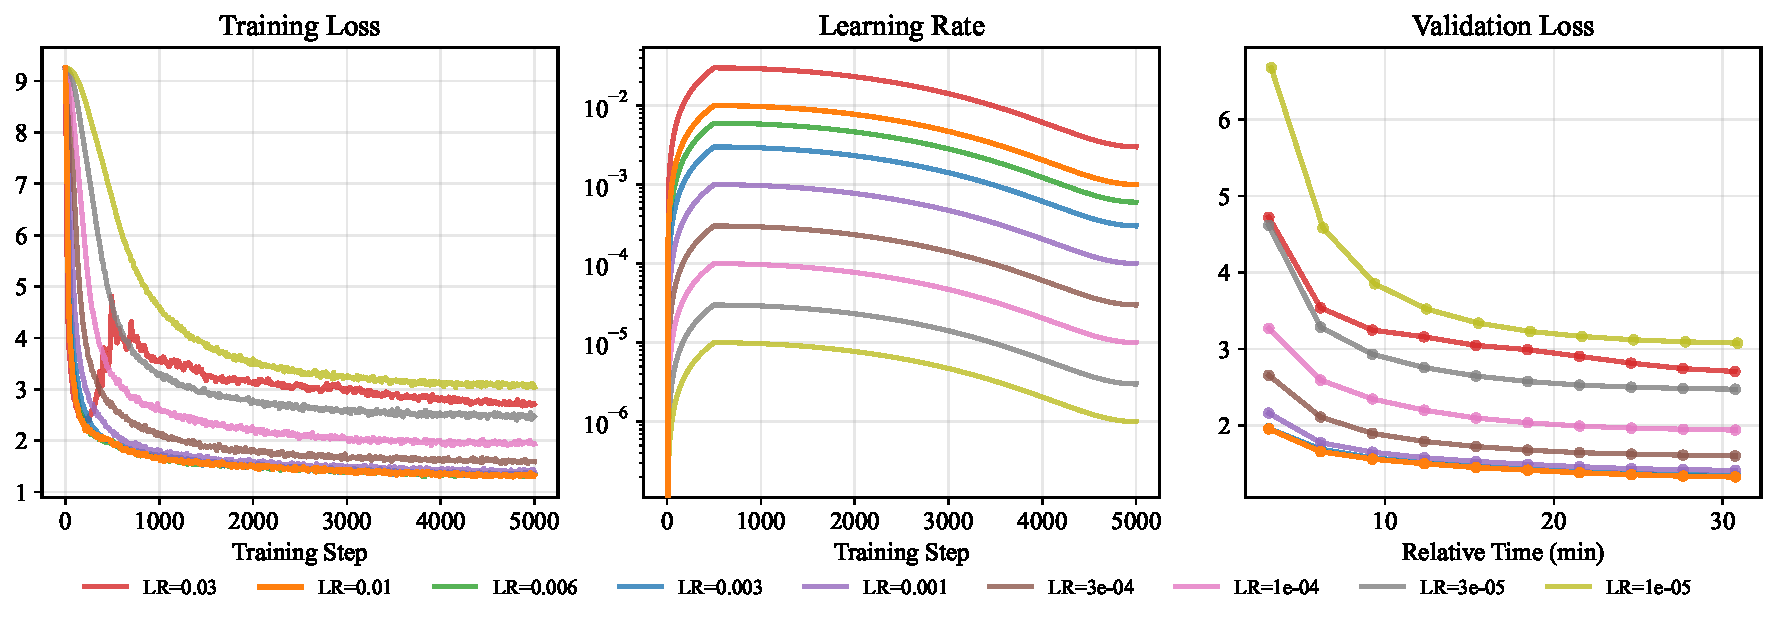
\includegraphics[width=\textwidth]{images/ts_learning_rate_experiments.pdf}
        \vspace{-20pt} % Reduce space between image and caption
        \caption{Learning rate experiments on TinyStories dataset}
        \label{fig:ts_learning_rate_experiments}
    \end{subfigure}
        
    \begin{subfigure}[t]{\textwidth}
        \centering
        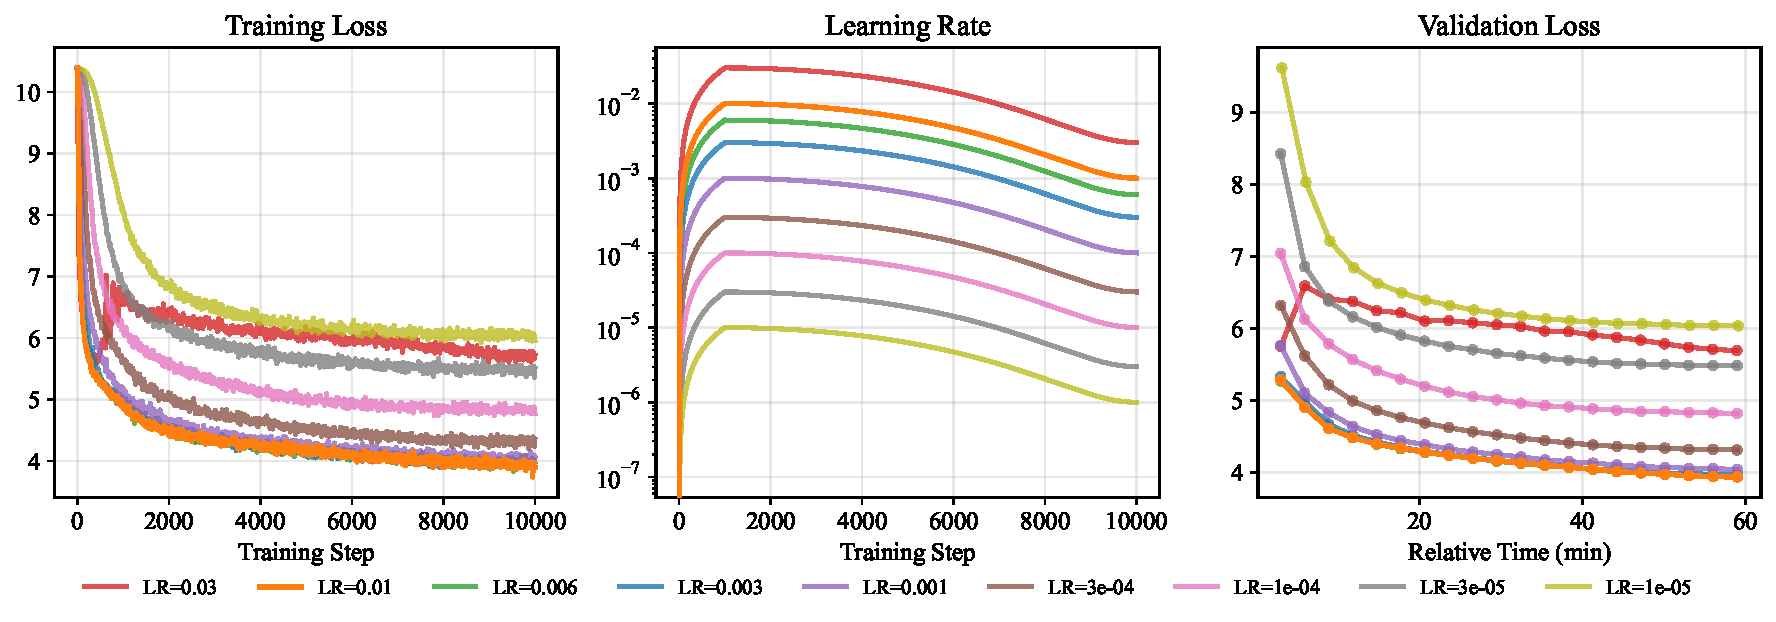
\includegraphics[width=\textwidth]{images/owt_learning_rate_experiments.pdf}
        \vspace{-20pt} % Reduce space between image and caption
        \caption{Learning rate experiments on OpenWebText dataset}
        \label{fig:owt_learning_rate_experiments}
    \end{subfigure}
    
    \caption{Learning rate experiments showing training loss (left), learning rate schedule (middle), and validation loss over time (right) for both datasets. The highlighted orange line represents LR=0.01, which achieved the best performance across both TinyStories and OpenWebText. Complete experiment logs/configs are available on the W\&B: \href{https://api.wandb.ai/links/donglinkang2021-beijing-institute-of-technology/jhz7fp86}{Report}.}
    \label{fig:learning_rate_experiments}
\end{figure}

Key findings from both experiments:

- ($\leq 3 \times 10^{-4}$): Stable convergence but inefficient training

- ($1 \times 10^{-3}$ to $1 \times 10^{-2}$): Best balance of convergence speed and stability

- $1 \times 10^{-2}$ achieved val/loss of 1.327, surpassing the target of 1.45 on TinyStories

- $3 \times 10^{-2}$ caused training collapse during warmup at step 480

- OpenWebText experiments mirrored TinyStories results, with $1 \times 10^{-2}$ yielding the best val/loss of 3.93

\textbf{Part (b):}
The "edge of stability" hypothesis suggests optimal learning rates exist just below the divergence threshold. My experiments support this principle:

- $3 \times 10^{-2}$ caused immediate instability during warmup

- $1 \times 10^{-2}$ (approximately 3$\times$ below divergence) achieved the best validation performance

\end{answer}

\problem{batch\_size\_experiment}{Batch size variations (1 point) (2 H100 hrs)}

Vary your batch size all the way from 1 to the GPU memory limit. Try at least a few batch sizes in between, including typical sizes like 64 and 128.

\textbf{Deliverable}: Learning curves for runs with different batch sizes. The learning rates should be optimized again if necessary.

\textbf{Deliverable}: A few sentences discussing of your findings on batch sizes and their impacts on training.

\begin{answer}
I conducted comprehensive batch size experiments on TinyStories, testing values from 1 to 1024: [1, 2, 4, 8, 16, 32, 64, 128, 256, 512, 768, 1024]. All experiments used learning rate $1 \times 10^{-3}$ (selected for better balance of convergence speed and stability), training for 10,000 iterations with the same total token count of 327,680,000 to ensure fair comparison. The learning curves are shown in Figure \ref{fig:batch_size_experiments}.

Key Findings:

- {Small (1-16)}: Exhibited high gradient noise, and increased wall-clock training time despite processing the same number of tokens

- {Optimal (128)}: Achieved the lowest val/loss efficiently (8.75 minutes for 10k iterations)

- {Near (32,64,256,512,768)}: Showed competitive performance, faster per-step computation(256-768)

- {Large (1024)}: Training collapsed, which exceeds memory capacity

\begin{figure}[!htb]
    \centering
    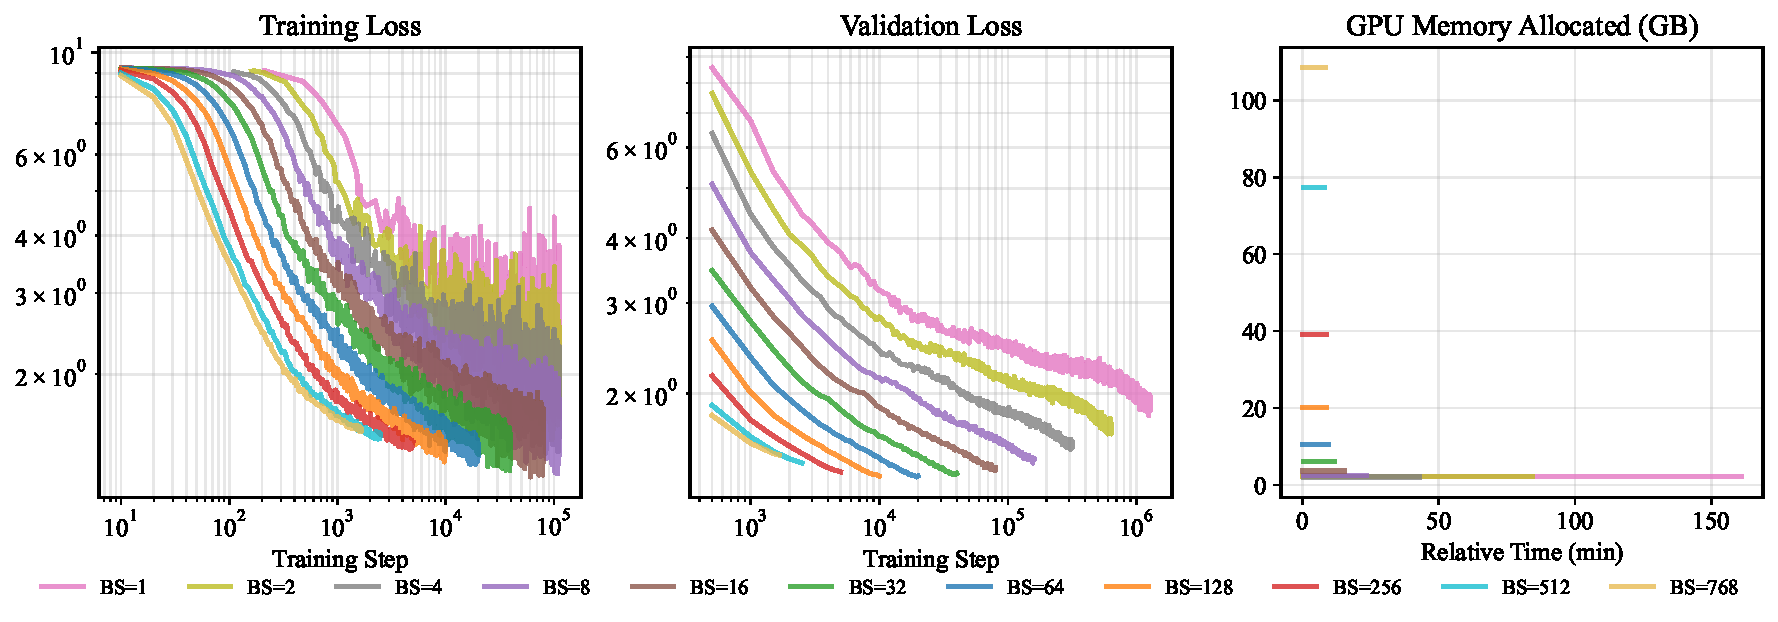
\includegraphics[width=\textwidth]{images/batch_size_experiments.pdf}
    \caption{Batch size experiments on TinyStories showing training loss vs. steps (left, log-log scale), validation loss vs. steps (middle, log-log scale), and GPU memory vs. time (right). Batch size 128 (orange line) achieved the best validation performance with only 8.75 minutes of training time for 10,000 iterations. Complete experiment logs are available on W\&B: \href{https://api.wandb.ai/links/donglinkang2021-beijing-institute-of-technology/ejo2bn9n}{Report}.}
    \label{fig:batch_size_experiments}
\end{figure}

\end{answer}

\problem{generate}{Generate text (1 point)}

Using your decoder and your trained checkpoint, report the text generated by your model. You may need to manipulate decoder parameters (temperature, top-$p$, etc.) to get fluent outputs.

\textbf{Deliverable}: Text dump of at least 256 tokens of text (or until the first \lstinline{<|endoftext|>} token), and a brief comment on the fluency of this output and at least two factors which affect how good or bad this output is.

\begin{answer}

Here is a sample of text generated by the best model(val/loss=1.327) from Learning rate experiments on the TinyStories dataset, using max generation length of 1000, a temperature of 0.6 and top-p sampling with p=0.95:

\begin{quote}
Once upon a time, there was a little girl named Lily. She had a doll that she loved very much. The doll was very pretty and expensive. Lily would play with her doll every day and take it with her everywhere she went. One day, Lily and her doll went to the park. They played on the swings and the slide. Lily was having so much fun that she forgot her doll at the park. She forgot about her doll at home. When it was time to go home, Lily's mom called her. Lily was sad because she forgot her doll at the park. She missed her doll and wished she had her doll back. The next day, Lily found her doll at the park and remembered her doll at the park. She ran back to the park and found her doll waiting for her. Lily was so happy to have her doll back and promised to always remember her. Once upon a time, there was a little girl named Sue. She loved to play with her toys and eat yummy food. One day, Sue saw a big, green avocado on the table. She wanted to eat it, but she knew she should ask her mom first. Sue went to her mom and said, "Mom, can I eat the avocado?" Her mom smiled and said, "Yes, you can eat the avocado, but be careful not to break it." Sue was very happy and started to eat the avocado. But then, something unexpected happened. The avocado started to talk! It said, "Please don't eat me!" Sue was very surprised. She did not eat the avocado, but she still loved it very much. Sue and the avocado became best friends. They played and lived happily ever after. Once upon a time, there was a little boy named Tim. He had a big, and he was very tired. He wanted to eat, but he could not. He tried to eat, but he was sad. He had a bad feeling. One day, a lot. She was so close to the day. She was very tired, but she was in the park. She went to the park. She was happy. One day, but a boy was not available. She was not fit in the next to. She went to the day. She felt very well. She was happy. She was a little bit. Once upon a time, there was a little boy, and she had a time. The little girl's house to play. She liked to play area to play. The park. She would go. The little boy's birthdays time to go, but she got a little girl's birthday party. At the park. The park. But, but the park. But, but she could not. She was in the park. She was in the park. The park. Sue's birthday party. Sue's birthday party. Sue's birthday. Sue's birthday to her birthday. At the park. Sue's birthday party. Once there was a big party time, and she had a new season. Sue's birthday, so her mom and her mom's things. Sue's birthdays value her mom's house. Sue, her mom said, her things, and they were not. One day, Sue. She was her house. Sue's birthday. Sue's home. Sue's birthday to go to go to go. Sue's home. Sue's house, but her house. Sue went to go. Sue's room was in a clear that she would be careful not be careful with her mom and she did not to have her mom said, "Mom said, it. Her mom was her mom said, "Please, but also had to remind her mom would not to be careful. She took her mom. She was not. Sue's room for too much better than before she could not. One day, she did not want to eat, "Hi, but not hungry. She said, but not hungry. She wanted her mom, but she would not eat, and she would not. She would open a lot of her mom was always be sad. One day, she was in the whole wide-evia. Avi-evid-so-b at the day. She knew that day. The sun, but the same food was a little boy's mom made a lot of her mom and her mom said thank you, and she thought about the day. Lily and she was a big, and she felt hungry. Lily's day, and her mom said, so much. Lily, but she was a big, and her mom's food to eat, but the day, but the day. Lily's food. The end, and she was not very hungry. Lily was full of a little, and her small, and her favorite food
\end{quote}

\textbf{Comment:}

The generated text shows mixed quality. The first two stories (Lily's doll and Sue's talking avocado) are coherent with proper grammar and logical plots. After ~200 tokens, quality degrades significantly with repetitive phrases ("Sue's birthday party"), incomplete sentences ("He had a big, and he was very tired"), and nonsense ("wide-evia. Avi-evid-so-b").

\textbf{Key factors affecting quality:}

The model uses a 256-token context window during training. Beyond this length, it loses track of earlier content, causing repetition and fragmentation. Maybe the TinyStories dataset contains mostly short stories (<300 tokens), so the model hasn't learned long-form generation. Additionally, with only 22M parameters, the model has limited capacity for complex linguistic patterns and long-range dependencies.

\end{answer}

\problem{layer\_norm\_ablation}{Remove RMSNorm and train (1 point) (1 H100 hr)}

Remove all of the RMSNorms from your Transformer and train. What happens at the previous optimal learning rate? Can you get stability by using a lower learning rate?

\textbf{Deliverable}: A learning curve for when you remove RMSNorms and train, as well as a learning curve for the best learning rate.

\textbf{Deliverable}: A few sentence commentary on the impact of RMSNorm.

\begin{answer}

I conducted comprehensive experiments removing RMSNorm from the Transformer architecture across three different learning rates: $1 \times 10^{-2}$, $1 \times 10^{-3}$, and $3 \times 10^{-4}$. The learning curves are shown in Figure~\ref{fig:rmsnorm_ablation_experiments}.

\textbf{Commentary:} RMSNorm is essential for training stability in Transformer architectures. Without it, training diverges catastrophically at the optimal learning rate ($1 \times 10^{-2}$), with losses exploding to over $10^{26}$ within hundreds of steps. While lower learning rates ($1 \times 10^{-3}$ and $3 \times 10^{-4}$) provide some stability, they converge to significantly worse solutions compared to models with RMSNorm. These results demonstrate that RMSNorm enables both efficient training with higher learning rates and better final model quality by maintaining well-conditioned gradients throughout training.

\begin{figure}[!htb]
    \centering
    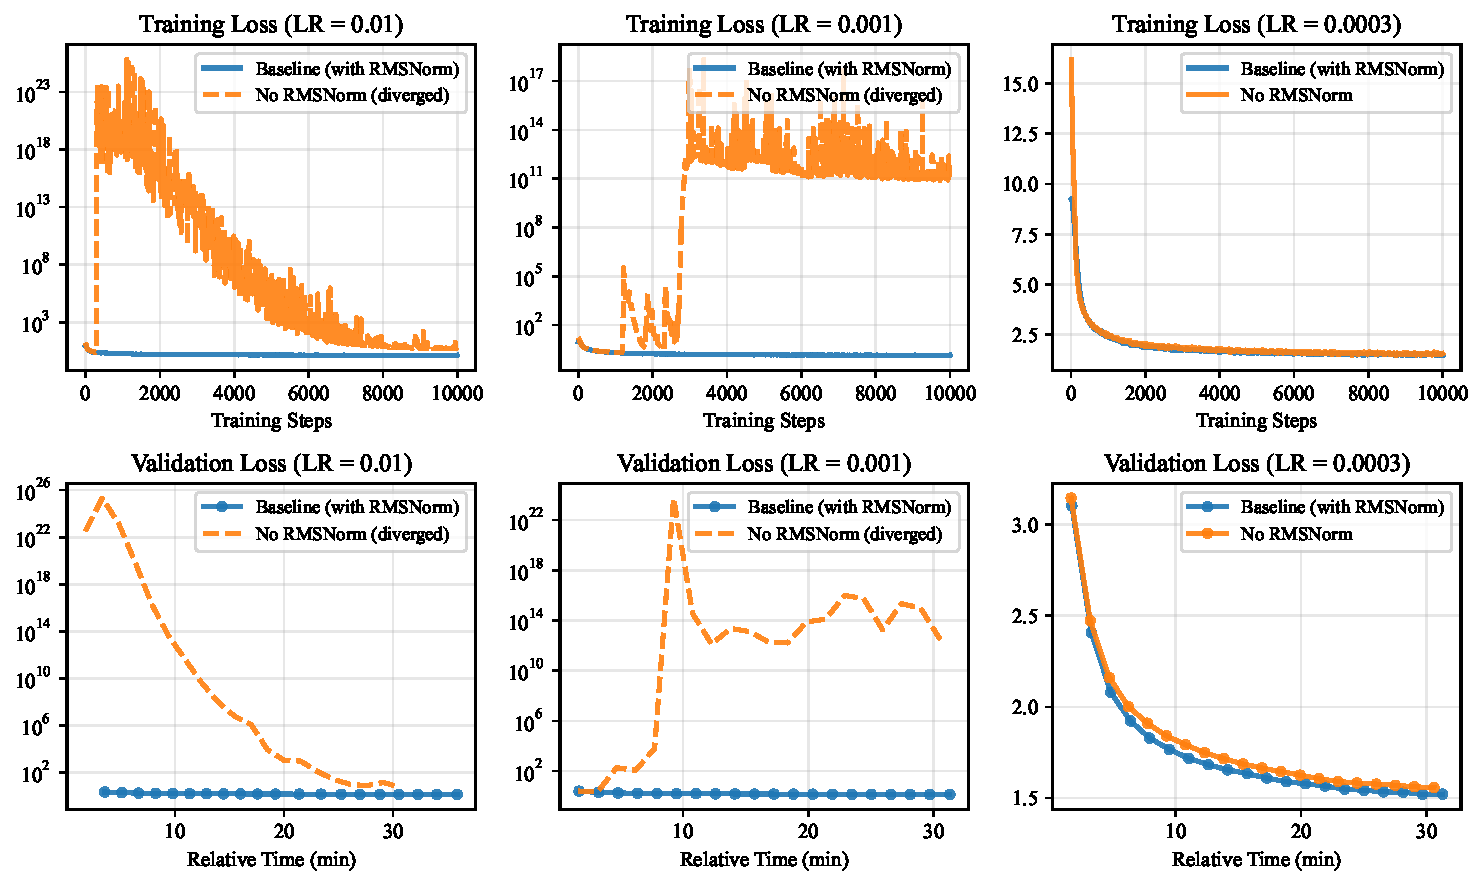
\includegraphics[width=\textwidth]{images/rmsnorm_ablation_experiments.pdf}
    \caption{RMSNorm ablation experiments comparing baseline (with RMSNorm) vs. no RMSNorm across different learning rates. Top row shows training loss vs. steps, bottom row shows validation loss vs. relative time.}
    \label{fig:rmsnorm_ablation_experiments}
\end{figure}

\end{answer}

\problem{pre\_norm\_ablation}{Implement post-norm and train (1 point) (1 H100 hr)}

Modify your pre-norm Transformer implementation into a post-norm one. Train with the post-norm model and see what happens.

\textbf{Deliverable}: A learning curve for a post-norm transformer, compared to the pre-norm one.

\begin{answer}

The learning curves are shown in Figure~\ref{fig:prenorm_ablation}.

\begin{figure}[!htb]
    \centering
    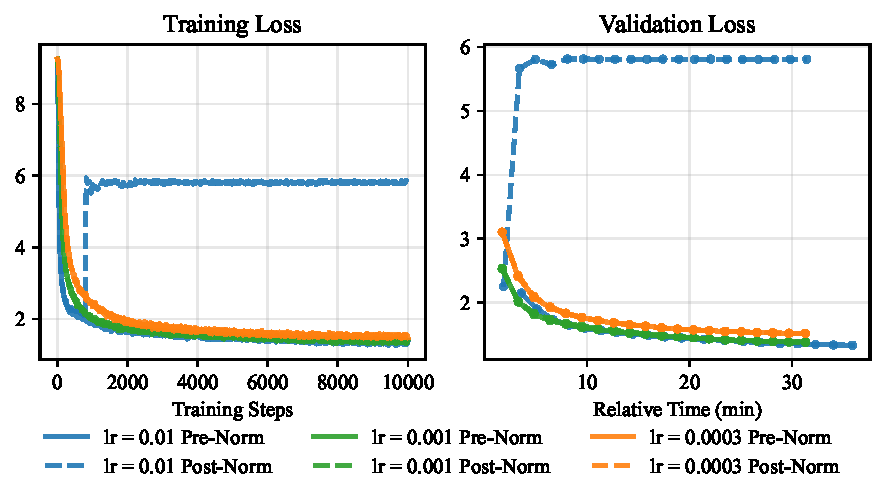
\includegraphics[width=0.6\textwidth]{images/prenorm_ablation_experiments.pdf}
    \caption{Training and validation loss for pre-norm vs. post-norm across multiple learning rates.}
    \label{fig:prenorm_ablation}
\end{figure}

\textbf{Commentary:} The pre-norm transformer remained stable across both learning rates, whereas the post-norm variant using the optimal learning rate diverged quickly, showing that pre-norm is more stable than post-norm.
\end{answer}

\problem{no\_pos\_emb}{Implement NoPE (1 point) (1 H100 hr)}

Modify your Transformer implementation with RoPE to remove the position embedding information entirely, and see what happens.

\textbf{Deliverable}: A learning curve comparing the performance of RoPE and NoPE.

\begin{answer}

The learning curves are shown in Figure~\ref{fig:rope_ablation}.

\begin{figure}[!htb]
    \centering
    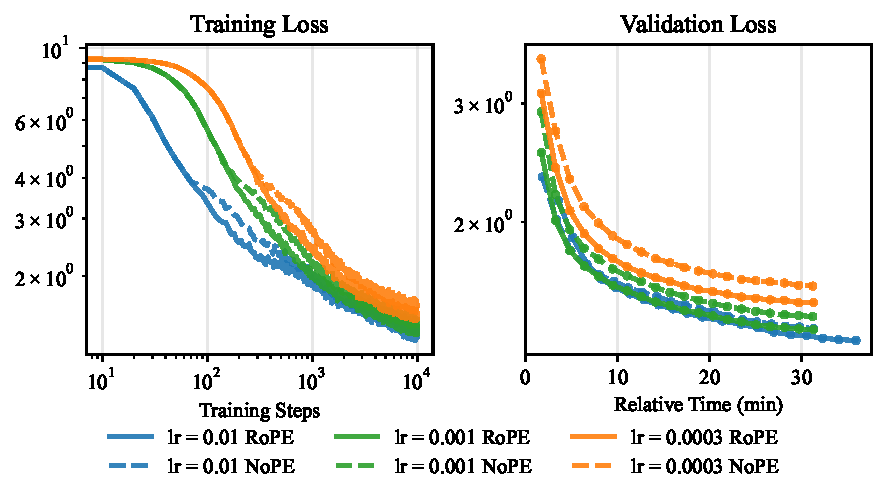
\includegraphics[width=0.6\textwidth]{images/rope_ablation_experiments.pdf}
    \caption{Training and validation loss for RoPE vs. NoPE across multiple learning rates.}
    \label{fig:rope_ablation}
\end{figure}

\textbf{Commentary:} RoPE maintained lower training and validation losses at every learning rate, while NoPE plateaued more quickly. This suggests that removing positional encodings limits convergence speed and final quality, even with conservative learning rate. However, the stability of NoPE at optimal learning rate 0.01 indicates that positional encodings are not strictly necessary for training stability, but they do enhance performance.

\end{answer}

\problem{swiglu\_ablation}{SwiGLU vs. SiLU (1 point) (1 H100 hr)}

\textbf{Deliverable}: A learning curve comparing the performance of SwiGLU and SiLU feed-forward networks, with approximately matched parameter counts.

\textbf{Deliverable}: A few sentences discussing your findings.

\begin{answer}

The learning curves \footnote{The ablation experiment logs/configs are available on W\&B: \href{https://api.wandb.ai/links/donglinkang2021-beijing-institute-of-technology/c54zgdnw}{Report}} are shown in Figure~\ref{fig:swiglu_ablation}.

\begin{figure}[!htb]
    \centering
    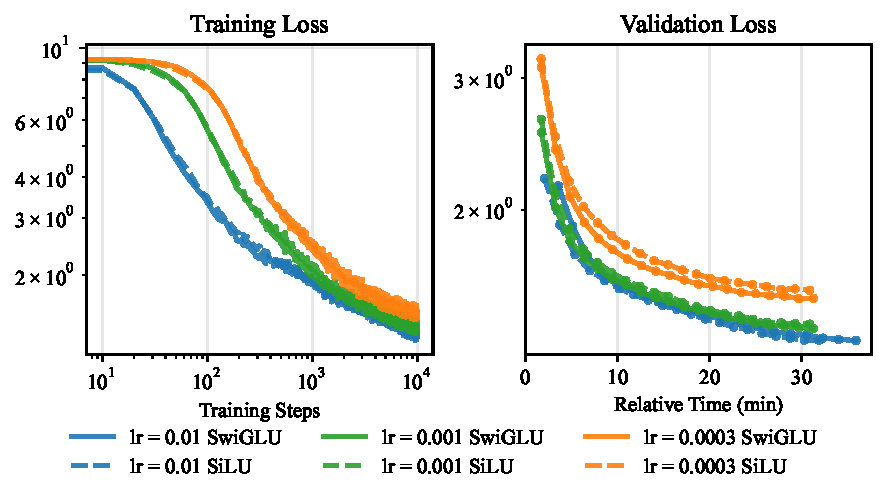
\includegraphics[width=0.6\textwidth]{images/swiglu_ablation_experiments.pdf}
    \caption{Training and validation loss for SwiGLU vs. SiLU across multiple learning rates.}
    \label{fig:swiglu_ablation}
\end{figure}

\textbf{Commentary:} SiLU edges out SwiGLU only at the optimal learning rate (0.01), delivering slightly lower losses. Across the stable learning-rate regime (0.001 and 0.0003), SwiGLU converges faster and finishes with better validation loss, indicating that the gating boost helps when optimization pressure is lower.

\end{answer}

\problem{main\_experiment}{Experiment on OWT (2 points) (3 H100 hrs)}

Train your language model on OpenWebText with the same model architecture and total training iterations as TinyStories. How well does this model do?

\textbf{Deliverable}: A learning curve of your language model on OpenWebText. Describe the difference in losses from TinyStories - how should we interpret these losses?

\textbf{Deliverable}: Generated text from OpenWebText LM, in the same format as the TinyStories outputs. How is the fluency of this text? Why is the output quality worse even though we have the same model and compute budget as TinyStories?

\begin{answer}

The learning curves\footnote{The main experiment logs/configs are available on W\&B: \href{https://api.wandb.ai/links/donglinkang2021-beijing-institute-of-technology/k1na9uic}{Report}.} comparing TinyStories and OpenWebText are shown in Figure~\ref{fig:main_experiments}.

\begin{figure}[!htb]
    \centering
    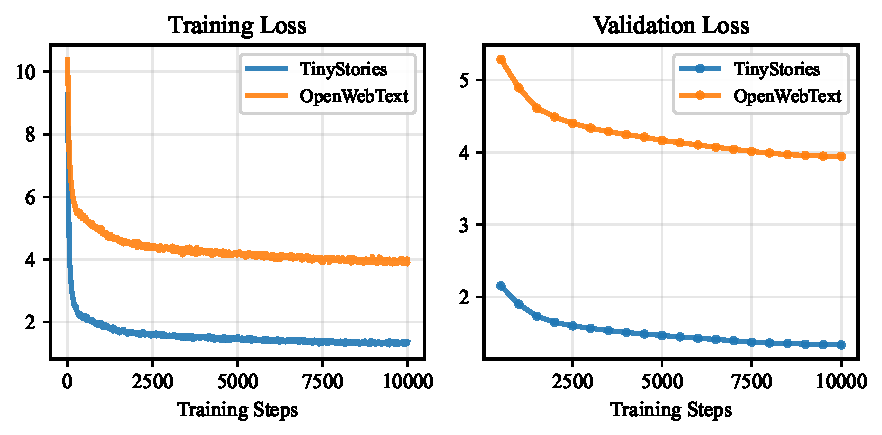
\includegraphics[width=0.6\textwidth]{images/main_experiments.pdf}
    \caption{Main experiments comparing TinyStories and OpenWebText datasets.}
    \label{fig:main_experiments}
\end{figure}

\textbf{Loss Difference:} The OpenWebText model achieves significantly higher losses compared to TinyStories across both training and validation. The final validation loss for OpenWebText is approximately 3.93, while TinyStories achieves 1.33. This difference reflects the inherent complexity of the datasets: OpenWebText contains diverse, real-world web content with complex vocabulary, grammar, and topics, whereas TinyStories consists of simple, repetitive children's stories with limited vocabulary and predictable structures.

\textbf{Generated Text:} Here is a sample of the first 1000 tokens generated by the OpenWebText model, using temperature 0.6 and top-p sampling with p=0.95:

\begin{quote}
The Miami Heat are a team of world champions, and the Heat are the same team that now will have their first team. The Heat are the team that has been known for their depth, but they are the team that will be getting their first team on Saturday. The Heat are the team that has been designated to the Heat in recent years, but that鈥檚 not the case. It鈥檚 not just the team that is building a roster that will be the NBA鈥檚 best-performing team, but it鈥檚 also the latest sports that will be the NBA鈥檚 first team in the NBA. This team is the team that is building a team that will be in the league. They will be making a team that will be able to compete in the playoffs. The Heat are the team that will be building the team鈥檚 best-performing team, and the team will have a chance to win the Heat鈥檚 first team in the series. The Heat are the team that will be in the NBA, and they are going to be the team that will be the team that will be the next best team in the series. The Heat are the team that will be the team that will be the team that will be the team that will be the team鈥檚 best team. The Heat will have a team that will be the team that will be the team that will be the team that will be the team that will be the team. When you guys are the team that has to play the Heat. They鈥檙e in the Heat, and the Heat have the best team that can beat the Heat in the Bulls and the Heat are the team. They鈥檝e got the team that has the most of which is the team that team, and they. Saints, the Heat fans. I鈥檚 Wright W A This The K B K It LSU G. Cous The The The If The R The The It The The It The The The It鈥檚 The The The The The The The The The The The The We鈥檚 The The The The The The The next The The The It鈥檚 Lets The The It鈥檚 The The The second The The only The The best The next- The The It鈥檛 They鈥橳ight- It鈥檚 The entire It鈥橫unoby A lot of The next of The other The same-Bened A/fresh The two- 鈥淚鈥橳he other players鈥滻鈥橧 think 鈥淭he best of the last year-Diamen. the best. the first- the 鈥淭he best-t. I think of the game and it鈥橳he most 鈥淭he second- playing the other than
\end{quote}

\textbf{Output Fluency:} The OpenWebText model exhibits significantly degraded output quality compared to TinyStories. The text demonstrates severe coherence issues, including excessive repetition (e.g., "the team that") and grammatical inconsistencies. The garbled characters (e.g., \lstinline{It鈥檚} for \lstinline{It’s}) are a known encoding artifact, which is further discussed in the Appendix~\ref{appendix:error-encoding}.

Four key factors explain this quality degradation:

\textbf{1. Vocabulary Size:} OpenWebText uses a vocabulary of ~32,000 tokens, far larger than TinyStories' ~10,000. The 22M-parameter model lacks the capacity to effectively model this larger linguistic space. An experiment reducing OpenWebText's vocabulary to 10,000 confirmed this, yielding better results.

\textbf{2. Training Data:} OpenWebText is scraped from the web and contains significant noise, whereas TinyStories is synthetically generated and clean. This difference in data quality directly impacts the model's ability to learn coherent language patterns.

\textbf{3. Context Window:} The model was trained with a 256-token context window. When asked to generate text far exceeding this length (1000 tokens), the model loses track of long-range dependencies, leading to degenerative repetition. This is analogous to long-horizon forecasting in RNNs, where predictions can collapse to a constant value.

\textbf{4. Training Inefficiency:} With an identical token budget, the model trained on OpenWebText sees fewer examples per concept/task due to the dataset's diversity. In contrast, TinyStories' simpler, repetitive structure allows for more robust pattern learning within the same compute budget.

\end{answer}

\problem{leaderboard}{Leaderboard (6 points) (10 H100 hrs)}

You will train a model under the leaderboard rules above with the goal of minimizing the validation loss of your language model within 1.5 H100-hour.

\textbf{Deliverable}: The final validation loss that was recorded, an associated learning curve that clearly shows a wallclock-time x-axis that is less than 1.5 hours and a description of what you did. We expect a leaderboard submission to beat at least the naive baseline of a 5.0 loss. Submit to the leaderboard here: \url{https://github.com/stanford-cs336/assignment1-basics-leaderboard}.

\begin{answer}

\textbf{Final Result:} I achieved a validation loss of \textbf{3.335} at the 90-minute mark, ranking \textbf{24th} on the global leaderboard\footnote{Leaderboard: \url{https://github.com/stanford-cs336/assignment1-basics-leaderboard}}. The learning curves are shown in Figure~\ref{fig:leaderboard_experiments}.

\begin{figure}[!htb]
    \centering
    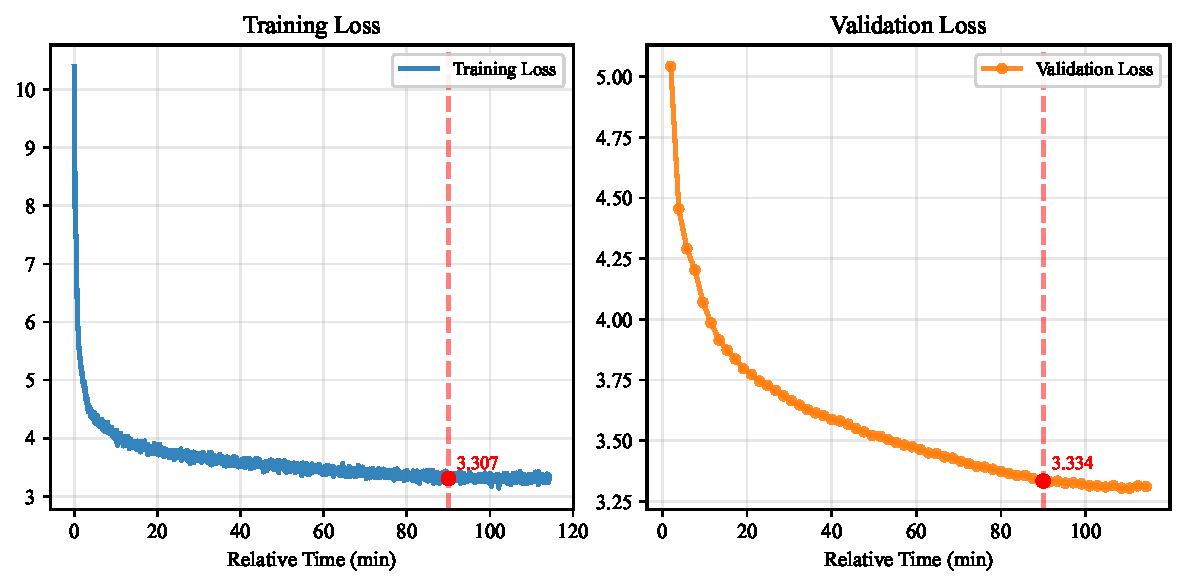
\includegraphics[width=0.8\textwidth]{images/leaderboard_experiments.pdf}
    \caption{Leaderboard submission learning curves showing training loss (left) and validation loss (right) vs. relative time in minutes. The red dashed line marks the 90-minute budget limit, with the final validation loss of 3.335 annotated.}
    \label{fig:leaderboard_experiments}
\end{figure}

\textbf{Key Modifications:}

Within the constraints of 80GB GPU memory and 1.5-hour wall-clock time using only the OpenWebText training set, I implemented the following modifications:

- \textbf{Model Size:} Scaled up to GPT-2 Small size (d\_model=768, d\_ff=2048, n\_head=12, n\_layer=12)

- \textbf{QK Normalization:} Added RMSNorm to query and key projections before RoPE for stability

- \textbf{Muon Optimizer:} Adopted the Muon optimizer (inspired by modded-nanogpt) for  efficient optimization

- \textbf{Weight Tying:} Tied the token embedding and output projection weights

- \textbf{LR Schedule:} Used cosine annealing from 1e-2 to 0 over 30,000 iterations with 2,000 warmup steps

\textbf{Ablation Study:}

Table~\ref{tab:leaderboard_ablations} summarizes the impact of each modification on validation loss:

\begin{table}[!htb]
\centering
\caption{Ablation study showing the impact of different modifications on validation loss.}
\label{tab:leaderboard_ablations}
\begin{tabular}{lcc}
\toprule
\textbf{Configuration} & \textbf{Val Loss - Min} & \textbf{$\Delta$ Loss} \\
\midrule
\multicolumn{3}{l}{\textit{Model Size}} \\
\addlinespace[0.5ex]
Baseline (d\_model=512, n\_layer=4) & 3.695 & - \\
GPT-2 Small (d\_model=768, n\_layer=12) & 3.335 & -0.360 \\
GPT-2 Small + (n\_layer=16) & 3.264 & -0.071 \\
\addlinespace[1ex]
\multicolumn{3}{l}{\textit{Optimizer \& Learning Rate (GPT-2 Small)}} \\
\addlinespace[0.5ex]
AdamW (lr=1e-3) & 3.482 & - \\
AdamW (lr=1e-2) & 3.436 & -0.046 \\
AdamW (lr=1e-3) + Muon (lr=3e-2) & 3.454 & -0.028 \\
AdamW (lr=1e-2) + Muon (lr=3e-2) & 3.427 & -0.055 \\
\addlinespace[1ex]
\multicolumn{3}{l}{\textit{Weight Tying}} \\
\addlinespace[0.5ex]
Baseline w/o weight tying & 3.753 & - \\
Baseline w/ weight tying & 3.695 & -0.058 \\
GPT-2 Small w/o weight tying & 3.427 & - \\
GPT-2 Small w/ weight tying & 3.362 & -0.065 \\
\bottomrule
\end{tabular}
\end{table}

\textbf{Analysis:}

The most significant improvement ($\Delta = -0.360$) came from scaling to GPT-2 Small architecture, demonstrating that model capacity is crucial given sufficient compute budget. Weight tying consistently improved performance across model sizes ($\Delta \approx -0.06$), reducing parameter count while maintaining expressiveness. The Muon optimizer combined with higher learning rates showed modest gains over AdamW alone. QK normalization provided training stability without degrading final performance. Further scaling to 16 layers showed additional gains but exceeded the 90-minute time budget.

\end{answer}



\bibliographystyle{plainnat}
\bibliography{ref}

\newpage
\appendix
\section{Appendix}

\subsection{Parameter Calculation Verification}
\label{appendix:param-verification}

To verify that our parameter calculation formula is correct, we provide the following verification code that compares the actual parameter count from a PyTorch model (implemented in \texttt{cs336\_basics/model.py}) with our analytical formula:

\begin{lstlisting}[language=Python, caption={Parameter count verification code}]
from cs336_basics.model import TransformerLM

model_cfg = dict(
    vocab_size=10000,
    context_length=256,
    d_model=512,
    num_layers=4,
    num_heads=16,
    d_ff=1344, 
    rope_theta=10000,
)

model = TransformerLM(**model_cfg)
total_params = sum(p.numel() for p in model.parameters())

def compute_model_size_from_scratch(
    vocab_size: int,
    context_length: int,
    d_model: int,
    num_layers: int,
    num_heads: int,
    d_ff: int,
    **kwargs
):
    total_params = 0
    total_params += vocab_size * d_model  # token embedding
    total_params += num_layers * ( # per block
        4 * (d_model * d_model) +  # Q, K, V, O projections
        3 * (d_model * d_ff) +     # SwiGLU layers
        2 * (d_model)              # RMSNorm layers
    )
    total_params += d_model  # final RMSNorm
    total_params += d_model * vocab_size  # output projection
    return total_params

print(f"Total number of parameters: {total_params}")     
print("Computed model size from scratch:", compute_model_size_from_scratch(**model_cfg))
\end{lstlisting}

\begin{lstlisting}
Total number of parameters: 22696448
Computed model size from scratch: 22696448
\end{lstlisting}

\subsection{Memory Calculation Verification}
\label{appendix:memory-verification}

\begin{lstlisting}
def compute_model_size(
    vocab_size: int,
    context_length: int,
    d_model: int,
    num_layers: int,
    num_heads: int,
    d_ff: int,
    **kwargs
):
    total_params = 0
    total_params += vocab_size * d_model  # token embedding
    total_params += num_layers * ( # per block
        4 * (d_model * d_model) +  # Q, K, V, O projections
        3 * (d_model * d_ff) +     # SwiGLU layers
        2 * (d_model)              # RMSNorm layers
    )
    total_params += d_model  # final RMSNorm
    total_params += d_model * vocab_size  # output projection
    return total_params

def compute_memory(vocab_size: int,
    context_length: int,
    d_model: int,
    num_layers: int,
    num_heads: int,
    d_ff: int,
    batch_size: int,
    **kwargs
) -> float:
    param_size = compute_model_size(vocab_size, context_length, d_model, num_layers, num_heads, d_ff)
    optimizer_size = param_size * 3  # Adam optimizer
    activation_size = batch_size * context_length *(
        num_layers * (
            8 * d_model + 2 * d_ff + 2 * num_heads * context_length
        ) + d_model + 2 * vocab_size  
    )
    memory_bytes = (param_size + optimizer_size + activation_size) * 4  # assuming 4 bytes per parameter (float32)
    return memory_bytes / (1024 ** 3)  # convert to GB


if __name__ == "__main__":
    # GPT-2 XL
    cfg = dict(
        vocab_size=50257,
        context_length=1024,
        d_model=1600,
        num_layers=48,
        num_heads=25,
        d_ff=6400, 
        rope_theta=10000,
        batch_size=3.34,
    )
    model_size = compute_model_size(**cfg)
    memory_gb = compute_memory(**cfg)
    print(f"Model size: {model_size/(1e9):.2f}B parameters")
    print(f"Estimated memory usage during training: {memory_gb:.2f} GB")
\end{lstlisting}

\begin{lstlisting}
Model size: 2.13B parameters
Estimated memory usage during training: 79.97 GB
\end{lstlisting}

\subsection{GPT-2 FLOP Breakdown Code}
\label{appendix:gpt2-flop-breakdown}

To verify our FLOP breakdown for GPT-2 models, we provide the following code that computes the FLOP counts for attention, feed-forward, and language modeling head components based on the GPT-2 architecture:

\begin{lstlisting}
def compute_gpt2_flops(d_model:int, n_layer:int, T:int=1024) -> dict:
    d_ff = 4 * d_model
    vocab_size = 50_257
    attn_flops = 4 * 2 * T * d_model * d_model + 2 * 2 * T * T * d_model
    ff_flops = 3 * 2 * T * d_model * d_ff
    lm_head_flops = 2 * T * d_model * vocab_size
    total_flops = n_layer * (attn_flops + ff_flops) + lm_head_flops
    return {
        "attention": n_layer * attn_flops / total_flops,
        "feed-forward": n_layer * ff_flops / total_flops,
        "lm-head": lm_head_flops / total_flops,
        "total": total_flops / 1e12, # in TFLOPs
    }, {
        "attention": n_layer * attn_flops / 1e12,
        "feed-forward": n_layer * ff_flops / 1e12,
        "lm-head": lm_head_flops / 1e12,
        "total": total_flops / 1e12,
    }

print("GPT-2 small", compute_gpt2_flops(768, 12))
print("GPT-2 medium", compute_gpt2_flops(1024, 24))
print("GPT-2 large", compute_gpt2_flops(1280, 36))
print("GPT-2 XL", compute_gpt2_flops(1600, 48))
print("GPT-2 XL", compute_gpt2_flops(1600, 48, 16384))
\end{lstlisting}

\begin{lstlisting}
GPT-2 small ({'attention': 0.276396942718713, 'feed-forward': 0.49751449689368343, 'lm-head': 0.22608856038760353, 'total': 0.349630365696}, {'attention': 0.09663676416, 'feed-forward': 0.173946175488, 'lm-head': 0.079047426048, 'total': 0.349630365696})
GPT-2 medium ({'attention': 0.29932707434661254, 'feed-forward': 0.5986541486932251, 'lm-head': 0.1020187769601624, 'total': 1.033109504}, {'attention': 0.309237645312, 'feed-forward': 0.618475290624, 'lm-head': 0.105396568064, 'total': 1.033109504})
GPT-2 large ({'attention': 0.2996151010432329, 'feed-forward': 0.6420323593783562, 'lm-head': 0.05835253957841083, 'total': 2.2577545216}, {'attention': 0.67645734912, 'feed-forward': 1.4495514624, 'lm-head': 0.13174571008, 'total': 2.2577545216})
GPT-2 XL ({'attention': 0.29440647731422626, 'feed-forward': 0.6691056302596051, 'lm-head': 0.036487892426168594, 'total': 4.5133365248}, {'attention': 1.3287555072, 'feed-forward': 3.01989888, 'lm-head': 0.1646821376, 'total': 4.5133365248})    
GPT-2 XL ({'attention': 0.65922723665908, 'feed-forward': 0.32315060620543135, 'lm-head': 0.017622157135488675, 'total': 149.5227957248}, {'attention': 98.5694994432, 'feed-forward': 48.31838208, 'lm-head': 2.6349142016, 'total': 149.5227957248})
\end{lstlisting}

\subsection{Comparison of GPT-2 Parameter Counts with original paper}
\label{appendix:gpt2-param-comparison}

To verify our GPT-2 parameter count calculations, we provide the following comparison with the original GPT-2 paper~\cite{radford2019language}:

\begin{table}[h]
    \centering
    \caption{Comparison of our GPT-2 calculations with values reported in the original GPT-2 paper~\cite{radford2019language}.}
    \label{tab:gpt2-param-comparison}
    \begin{tabular}{c|c|c|c|c}
        \toprule
        Model & Our Calculation & Paper Reported & Difference & Relative Error \\
        \midrule
        GPT-2 Small & 124M & 117M & +7M & 5.98\% \\
        GPT-2 Medium & 354M & 345M & +9M & 2.61\% \\
        GPT-2 Large & 772M & 762M & +10M & 1.31\% \\
        GPT-2 XL & 1555M & 1542M & +13M & 0.84\% \\
        \bottomrule
    \end{tabular}
\end{table}

\begin{lstlisting}
def compute_gpt2_params(d_model:int, num_layers:int) -> float:
    vocab_size = 50_257
    d_ff = 4 * d_model
    total_params = 0
    total_params += vocab_size * d_model  # token embedding
    total_params += num_layers * ( # per block
        4 * (d_model * d_model) +  # Q, K, V, O projections
        # 3 * (d_model * d_ff) +     # our SwiGLU layers
        2 * (d_model * d_ff) +     # original gpt-2 layers
        2 * (d_model)              # RMSNorm layers
    )
    total_params += d_model  # final RMSNorm
    # total_params += d_model * vocab_size  # output projection tied with input embedding
    return total_params


print("GPT-2 small", compute_gpt2_params(768, 12) / 1e6, "M params")
print("GPT-2 medium", compute_gpt2_params(1024, 24) / 1e6, "M params")
print("GPT-2 large", compute_gpt2_params(1280, 36) / 1e6, "M params")
print("GPT-2 XL", compute_gpt2_params(1600, 48) / 1e9, "B params")
\end{lstlisting}

\begin{lstlisting}
GPT-2 small 123.551232 M params
GPT-2 medium 353.503232 M params
GPT-2 large 772.2112 M params
GPT-2 XL 1.5551264 B params
\end{lstlisting}

\subsection{Comprehensive Logging Code Snippet}
\label{appendix:logging-code}

\begin{lstlisting}
# Training script with comprehensive logging infrastructure
import hydra
from cs336_basics.logger import Logger
from cs336_basics.config import TrainConfig

@hydra.main(config_path="conf", config_name="train_config", version_base=None)
def main(cfg: TrainConfig) -> None:
    # Initialize logger with Hydra configuration
    logger = Logger(cfg)
    output_dir = Path(HydraConfig.get().runtime.output_dir)
    
    # ... model and data setup ...
    
    # Training loop with comprehensive logging
    for it in tqdm(range(start_iter, cfg.training.max_iters), desc="Training"):
        # ... forward/backward pass ...
        
        # Training metrics logging
        if it % cfg.training.log_interval == 0:
            ent = compute_entropy_chunked(logits).mean()
            logger.log_metrics({
                'train/loss': loss.item(), 
                'train/ppl': loss.exp().item(),
                'train/lr': lr,
                'train/entropy': ent.item(),
                'train/grad_norm': grad_norm
            }, step=it)
            
        # Validation logging
        if it % cfg.training.eval_interval == 0:
            metrics = evaluate(model, val_data, cfg, device)
            logger.log_metrics({
                'val/loss': metrics['val/loss'],
                'val/ppl': metrics['val/ppl'], 
                'val/entropy': metrics['val/entropy']
            }, step=it)
    
    # Log generated text samples
    generated_output = generate_text(model, tokenizer, ...)
    logger.log_text("Generated Text", generated_output, step=cfg.training.max_iters)
    
    logger.close()
    # Save final configuration
    OmegaConf.save(cfg, output_dir / 'config.yaml')

@torch.no_grad()
def evaluate(model, data, cfg, device):
    """Evaluation with entropy and perplexity tracking."""
    # ... evaluation loop ...
    return {
        'val/loss': mean_loss,
        'val/ppl': np.exp(mean_loss),
        'val/entropy': np.mean(entropies)
    }
\end{lstlisting}

\subsection{Analysis of the Error encodings 鈥檚}
\label{appendix:error-encoding}

To investigate the source of the garbled characters like \lstinline{鈥檚} in the generated text, I analyzed the raw training data (\lstinline{owt_train.txt}), the tokenizer's behavior, and the processed binary data (\lstinline{train.bin}). My goal was to understand the frequency and representation of different apostrophe styles.

The Python snippet below confirms the root cause: the sequence \lstinline{鈥檚} is the result of incorrectly decoding a UTF-8 encoded string \lstinline{’s} (using a right single quotation mark) with a different encoding, such as GBK.

\begin{lstlisting}
>>> "NBA’s".encode("utf-8").decode("utf-8")
'NBA’s'
>>> "NBA’s".encode("utf-8").decode("gbk")
'NBA鈥檚'
\end{lstlisting}

To quantify the presence of this error in the dataset, I ran scripts to count the occurrences of different \lstinline{'s} variants both in the raw text file and in the tokenized training data\footnote{The code for this analysis can be found in \href{https://github.com/donglinkang2021/cs336-assignment1-basics/blob/main/data_utils/count_word_from_train_txt.sh}{\lstinline{count_word_from_train_txt.sh}} and \href{https://github.com/donglinkang2021/cs336-assignment1-basics/blob/main/data_utils/count_word_from_train_bin.py}{\lstinline{count_word_from_train_bin.py}}.}.

\begin{lstlisting}
(cs336-basics) [root:assignment1-basics]$ python data_utils/count_word_from_train_bin.py 
============================================================
Token Sequence Occurrence Counting Tool
============================================================
Loading tokenizer: hf_tokenizer/openwebtext-32k/tokenizer.json
'鈥檚' -> token_ids: [164, 187, 99, 161, 104, 205]
''s' -> token_ids: [382]
'’s' -> token_ids: [286, 83]
'‘s' -> token_ids: [4719, 83]
------------------------------------------------------------
File size: 5.08 GB
Total tokens: 2,727,044,684
Target token sequences:
  '鈥檚': [164, 187, 99, 161, 104, 205]
  ''s': [382]
  '’s': [286, 83]
  '‘s': [4719, 83]
Start counting...
Counting progress: 100%|██████████████████████████████████| 2727044684/2727044684 [03:48<00:00, 11959960.05tokens/s]

Counting results:
----------------------------------------
'鈥檚' (sequence: [164, 187, 99, 161, 104, 205]): 2 times
''s' (sequence: [382]): 8,062,975 times
'’s' (sequence: [286, 83]): 11,253,531 times
'‘s' (sequence: [4719, 83]): 24,540 times

Total tokens: 2,727,044,684
Processing time: 228.02 seconds
============================================================
(cs336-basics) [root:assignment1-basics]$ bash data_utils/count_word_from_train_txt.sh 
Counting character occurrences in data/owt_train.txt...
File size: 12G
Occurrences of '鈥檚'
2
Occurrences of ''s'
8131046
Occurrences of '’s'
11277977
Occurrences of '‘s'
71423

Counting completed!
\end{lstlisting}

\textbf{Some Findings:}

The results from both the raw text and the tokenized data are consistent. They reveal that the dataset is dominated by standard apostrophes, with \lstinline{’s} (right single quote) being the most frequent variant (over 11 million times), followed by \lstinline{'s} (straight quote, over 8 million times).

Crucially, the garbled sequence \lstinline{鈥檚} appears only twice in the entire 12GB dataset. This confirms that the issue is not widespread data corruption but rather a rare artifact, likely from the original web scraping process.

The paradox that the model reproduces this extremely rare pattern invites some interesting speculation. Here are a couple of my hypotheses:

\textbf{1. Sensitivity to Low-Probability Patterns:} This behavior might indicate that the model is highly sensitive to every pattern it has learned, even those with vanishingly low probabilities. During a degenerative state where the model loses long-range context, it might latch onto any learned sequence that fits the immediate context. The fact that it can recall and repeat a pattern seen only twice suggests that no training example is truly forgotten, merely assigned a low probability.

\textbf{2. Preference for Longer Token Sequences:} An alternative hypothesis is that the model may develop a preference for longer token sequences to fulfill certain grammatical roles. The garbled \lstinline{鈥檚} is tokenized into a sequence of six tokens, whereas the correct \lstinline{'s} and \lstinline{’s} are tokenized into one and two tokens, respectively. It's conceivable that when the model is struggling to form a possessive, it defaults to a longer, more "descriptive" token sequence it has learned, even if it's incorrect. This is a fascinating thought, as it might offer a glimpse into why techniques like Chain-of-Thought (CoT) are effective—they guide the model to solve problems through longer, more deliberate sequences of tokens.


\end{document}